\documentclass[twocolumn,showpacs,pre,preprintnumbers,floatfix]{revtex4-1}
\usepackage{graphicx}
\usepackage[english]{babel}
\usepackage{amssymb}
\usepackage{amsbsy}
\usepackage{amsmath}
\usepackage{color}
\usepackage{natbib}
\usepackage{tikz,pgfplots}
\usetikzlibrary{spy}

\newcommand{\todo}[1]{ \fbox{{\bf TODO:} \color{red} #1}}
\newcommand{\ff}{{\mathbf{f}}}
\newcommand{\nn}{{\mathbf{n}}}
\newcommand{\rr}{{\mathbf{r}}}
\newcommand{\ssigma}{{\boldsymbol{\sigma}}}
\newcommand{\uu}{{\mathbf{u}}}
\newcommand{\xx}{{\mathbf{x}}}
\newcommand{\yy}{{\mathbf{y}}}
\newcommand{\grad}{{\triangledown}}
\newcommand{\bigO}{{\mathcal{O}}}
\renewcommand{\SS}{{\mathcal{S}}}
\newcommand{\DD}{{\mathcal{D}}}

\newif\ifTikz
%\Tikztrue
\Tikzfalse
% use these to not build the tikz images.  They take a while for the
% compiler to build.  If not using tikz, then it will use
% includegraphics with the pdf copy of the tikz.  These files will need
% updated as the tikz pictures are updated.  See how to use
% tikzexternalize below

%\usepgfplotslibrary{external}
%\tikzexternalize
% for turning tikz into pdf uncomment and run pdflatex -shell-escape
% 2dcomparison.tex


\begin{document}

\title{A comparative study of numerical and experimental viscous flow
in porous media}

\author{Pietro de Anna}
\email[E-mail: ]{pietrodeanna@gmail.com}
\affiliation{Massachusetts Institute of Technology}
\author{Bryan Quaife}
\email[E-mail: ]{quaife@ices.utexas.edu}
\affiliation{University of Texas}
\author{George Biros}
\affiliation{University of Texas}
\author{Ruben Juanes}
\affiliation{Massachusetts Institute of Technology}

\begin{abstract}
abstract
\end{abstract}

\maketitle

%%%%%%%%%%%%%%%%%%%%%%%%%%%%%%%%%%%%%%%%%%%%%%%%%%%%%%%%%%%%%%%%%%%%%%%%
{\em Introduction.}---We study things about porous flow.  Need to
discuss
\begin{itemize}
  \item Stokes assumption (small Reynold's number)
  \item 2D assumption
  \item Working with primitive variable instead of a homogenization such
  as Darcy's Law.
  \item Lagrangian coherent structures.
\end{itemize}
\begin{figure}[htps]
\ifTikz
\centering
  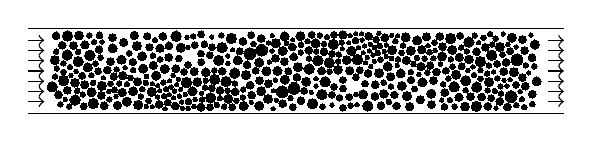
\begin{tikzpicture}[
  scale=2.0,
]

\foreach \y in {0.65,1.3,1.95,2.6,3.25,3.9,4.55}
  \draw[color=black,line width=0.5pt,solid,->]
    (0mm,\y mm) -- (1mm, \y mm);
% inlet arrows

\foreach \y in {0.65,1.3,1.95,2.6,3.25,3.9,4.55}
  \draw[color=black,line width=0.5pt,solid,->]
    (33mm,\y mm) -- (34mm, \y mm);
\filldraw[line width=0pt] (31.902159mm,4.8806829mm) circle (0.13975493mm);
\filldraw[line width=0pt] (10.132162mm,4.0931488mm) circle (0.13850288mm);
\filldraw[line width=0pt] (30.969474mm,4.1274072mm) circle (0.13908641mm);
\filldraw[line width=0pt] (30.444063mm,4.2913585mm) circle (0.13866492mm);
\filldraw[line width=0pt] (30.14856mm,4.9527324mm) circle (0.13939821mm);
\filldraw[line width=0pt] (21.259932mm,3.7576165mm) circle (0.13887385mm);
\filldraw[line width=0pt] (4.676123mm,4.4473972mm) circle (0.13874072mm);
\filldraw[line width=0pt] (8.94988mm,1.1012266mm) circle (0.13717489mm);
\filldraw[line width=0pt] (22.5929mm,3.8459084mm) circle (0.13785541mm);
\filldraw[line width=0pt] (8.674888mm,0.201377mm) circle (0.13905377mm);
\filldraw[line width=0pt] (14.143777mm,0.6118213mm) circle (0.13933866mm);
\filldraw[line width=0pt] (31.224078mm,1.2895281mm) circle (0.13886866mm);
\filldraw[line width=0pt] (15.487198mm,4.8442055mm) circle (0.13978215mm);
\filldraw[line width=0pt] (31.771043mm,2.4809153mm) circle (0.13963247mm);
\filldraw[line width=0pt] (9.40777mm,1.736749mm) circle (0.13883486mm);
\filldraw[line width=0pt] (9.770237mm,0.2365177mm) circle (0.13851263mm);
\filldraw[line width=0pt] (15.291087mm,3.166535mm) circle (0.13985378mm);
\filldraw[line width=0pt] (9.963742mm,1.1096327mm) circle (0.139531mm);
\filldraw[line width=0pt] (20.792104mm,1.1037774mm) circle (0.13884845mm);
\filldraw[line width=0pt] (24.789923mm,2.3812742mm) circle (0.13904318mm);
\filldraw[line width=0pt] (22.24938mm,4.9947966mm) circle (0.13915472mm);
\filldraw[line width=0pt] (27.901102mm,2.6268486mm) circle (0.13992071mm);
\filldraw[line width=0pt] (16.384172mm,4.3489007mm) circle (0.13858948mm);
\filldraw[line width=0pt] (19.927414mm,4.0145498mm) circle (0.13905697mm);
\filldraw[line width=0pt] (6.133579mm,2.8164537mm) circle (0.13918094mm);
\filldraw[line width=0pt] (7.864709mm,0.3344028mm) circle (0.13953435mm);
\filldraw[line width=0pt] (15.746136mm,0.743515mm) circle (0.13910904mm);
\filldraw[line width=0pt] (7.872138mm,1.7979244mm) circle (0.13890541mm);
\filldraw[line width=0pt] (15.540087mm,0.2021285mm) circle (0.13997894mm);
\filldraw[line width=0pt] (10.503964mm,0.348933mm) circle (0.13948045mm);
\filldraw[line width=0pt] (9.665134mm,1.437424mm) circle (0.13897064mm);
\filldraw[line width=0pt] (8.964672mm,1.9752671mm) circle (0.13826506mm);
\filldraw[line width=0pt] (10.063356mm,4.7419798mm) circle (0.13957932mm);
\filldraw[line width=0pt] (23.428188mm,2.9452357mm) circle (0.13903278mm);
\filldraw[line width=0pt] (21.650636mm,3.8707114mm) circle (0.13821651mm);
\filldraw[line width=0pt] (30.376882mm,1.6496325mm) circle (0.13876369mm);
\filldraw[line width=0pt] (9.729186mm,0.62528mm) circle (0.13702237mm);
\filldraw[line width=0pt] (23.061298mm,4.8612634mm) circle (0.13882079mm);
\filldraw[line width=0pt] (20.863424mm,0.4541594mm) circle (0.14019931mm);
\filldraw[line width=0pt] (20.958077mm,4.0872511mm) circle (0.1374433mm);
\filldraw[line width=0pt] (9.055093mm,1.5850561mm) circle (0.13888451mm);
\filldraw[line width=0pt] (11.641671mm,4.7642992mm) circle (0.1398072mm);
\filldraw[line width=0pt] (22.717519mm,3.5208726mm) circle (0.13908528mm);
\filldraw[line width=0pt] (8.332031mm,1.3492658mm) circle (0.13822887mm);
\filldraw[line width=0pt] (18.267159mm,1.6438743mm) circle (0.1394827mm);
\filldraw[line width=0pt] (20.420929mm,4.845512mm) circle (0.13885282mm);
\filldraw[line width=0pt] (19.2821mm,0.429216mm) circle (0.13947596mm);
\filldraw[line width=0pt] (21.189264mm,4.5690769mm) circle (0.1375947mm);
\filldraw[line width=0pt] (28.225031mm,2.8645929mm) circle (0.13940884mm);
\filldraw[line width=0pt] (12.660696mm,3.0865035mm) circle (0.13911386mm);
\filldraw[line width=0pt] (3.027663mm,2.5658623mm) circle (0.13973693mm);
\filldraw[line width=0pt] (15.2455mm,4.3875433mm) circle (0.13955092mm);
\filldraw[line width=0pt] (21.868004mm,3.6080242mm) circle (0.13842899mm);
\filldraw[line width=0pt] (12.967269mm,3.9467992mm) circle (0.13935437mm);
\filldraw[line width=0pt] (30.201523mm,2.0109952mm) circle (0.13833368mm);
\filldraw[line width=0pt] (25.824675mm,3.9003958mm) circle (0.13946036mm);
\filldraw[line width=0pt] (9.274736mm,1.3214113mm) circle (0.13898338mm);
\filldraw[line width=0pt] (21.95796mm,3.2181852mm) circle (0.13891933mm);
\filldraw[line width=0pt] (21.975109mm,4.0922893mm) circle (0.13832407mm);
\filldraw[line width=0pt] (12.655784mm,3.5517194mm) circle (0.13784076mm);
\filldraw[line width=0pt] (10.995816mm,1.1796195mm) circle (0.13946827mm);
\filldraw[line width=0pt] (26.167414mm,3.0309016mm) circle (0.13957932mm);
\filldraw[line width=0pt] (23.054766mm,3.3944572mm) circle (0.13966704mm);
\filldraw[line width=0pt] (10.58113mm,0.8005183mm) circle (0.13918194mm);
\filldraw[line width=0pt] (21.341521mm,4.1903308mm) circle (0.13880661mm);
\filldraw[line width=0pt] (30.583859mm,2.0508043mm) circle (0.13820135mm);
\filldraw[line width=0pt] (26.24731mm,0.751561mm) circle (0.13902785mm);
\filldraw[line width=0pt] (2.698244mm,2.3272574mm) circle (0.13896806mm);
\filldraw[line width=0pt] (29.68868mm,0.242872mm) circle (0.13919093mm);
\filldraw[line width=0pt] (20.781365mm,4.9687994mm) circle (0.13730916mm);
\filldraw[line width=0pt] (16.782393mm,4.5823074mm) circle (0.13856971mm);
\filldraw[line width=0pt] (28.580833mm,4.4033335mm) circle (0.13888821mm);
\filldraw[line width=0pt] (21.51524mm,3.456316mm) circle (0.13760099mm);
\filldraw[line width=0pt] (4.75741mm,2.1681228mm) circle (0.14010593mm);
\filldraw[line width=0pt] (9.214564mm,0.9012291mm) circle (0.13910975mm);
\filldraw[line width=0pt] (7.49626mm,2.2510825mm) circle (0.13905659mm);
\filldraw[line width=0pt] (18.261335mm,2.1102405mm) circle (0.13911007mm);
\filldraw[line width=0pt] (20.341497mm,4.3931356mm) circle (0.13850707mm);
\filldraw[line width=0pt] (7.481159mm,0.3510657mm) circle (0.13811751mm);
\filldraw[line width=0pt] (9.52004mm,2.0740332mm) circle (0.1392547mm);
\filldraw[line width=0pt] (23.43997mm,4.8413581mm) circle (0.13766145mm);
\filldraw[line width=0pt] (5.101877mm,1.2947471mm) circle (0.13952329mm);
\filldraw[line width=0pt] (21.735784mm,2.8830671mm) circle (0.13922453mm);
\filldraw[line width=0pt] (22.716201mm,4.2534265mm) circle (0.13834837mm);
\filldraw[line width=0pt] (29.534671mm,2.5453591mm) circle (0.1389823mm);
\filldraw[line width=0pt] (21.400171mm,3.1231763mm) circle (0.13889961mm);
\filldraw[line width=0pt] (15.559736mm,1.3448287mm) circle (0.13816319mm);
\filldraw[line width=0pt] (9.186667mm,2.3110442mm) circle (0.13975493mm);
\filldraw[line width=0pt] (9.585112mm,1.004652mm) circle (0.13785659mm);
\filldraw[line width=0pt] (21.154137mm,4.9600672mm) circle (0.13878263mm);
\filldraw[line width=0pt] (15.681852mm,2.0193019mm) circle (0.13939206mm);
\filldraw[line width=0pt] (21.710525mm,4.2967538mm) circle (0.13900826mm);
\filldraw[line width=0pt] (15.470186mm,3.8726582mm) circle (0.1399396mm);
\filldraw[line width=0pt] (5.557064mm,0.984788mm) circle (0.13856983mm);
\filldraw[line width=0pt] (2.340986mm,0.7942823mm) circle (0.13867249mm);
\filldraw[line width=0pt] (10.137902mm,0.2284164mm) circle (0.13801506mm);
\filldraw[line width=0pt] (17.956522mm,1.2474799mm) circle (0.13821955mm);
\filldraw[line width=0pt] (8.205326mm,0.9437805mm) circle (0.13919506mm);
\filldraw[line width=0pt] (8.206317mm,1.6734685mm) circle (0.13856183mm);
\filldraw[line width=0pt] (22.889491mm,0.6370575mm) circle (0.17558734mm);
\filldraw[line width=0pt] (23.018951mm,1.621364mm) circle (0.17491109mm);
\filldraw[line width=0pt] (24.669577mm,3.432819mm) circle (0.17408219mm);
\filldraw[line width=0pt] (4.254197mm,3.0684182mm) circle (0.17532075mm);
\filldraw[line width=0pt] (23.783605mm,4.2099249mm) circle (0.17554328mm);
\filldraw[line width=0pt] (29.316573mm,4.9471436mm) circle (0.17542089mm);
\filldraw[line width=0pt] (10.460252mm,4.8010144mm) circle (0.17514822mm);
\filldraw[line width=0pt] (26.667557mm,2.1263378mm) circle (0.1742936mm);
\filldraw[line width=0pt] (18.766931mm,4.3177115mm) circle (0.17352706mm);
\filldraw[line width=0pt] (22.307918mm,4.1898896mm) circle (0.17464248mm);
\filldraw[line width=0pt] (19.666447mm,3.2100202mm) circle (0.1747019mm);
\filldraw[line width=0pt] (20.465058mm,0.3932838mm) circle (0.17507576mm);
\filldraw[line width=0pt] (27.761746mm,1.3794262mm) circle (0.17614856mm);
\filldraw[line width=0pt] (13.631287mm,1.4239174mm) circle (0.17441716mm);
\filldraw[line width=0pt] (13.61728mm,0.9211878mm) circle (0.17359229mm);
\filldraw[line width=0pt] (3.989987mm,2.3288263mm) circle (0.17453846mm);
\filldraw[line width=0pt] (31.336718mm,0.8095166mm) circle (0.17467739mm);
\filldraw[line width=0pt] (2.221851mm,2.5388106mm) circle (0.17318612mm);
\filldraw[line width=0pt] (5.598661mm,2.70456mm) circle (0.17539442mm);
\filldraw[line width=0pt] (28.712823mm,2.1044988mm) circle (0.17424651mm);
\filldraw[line width=0pt] (29.667097mm,4.6605861mm) circle (0.17588718mm);
\filldraw[line width=0pt] (12.15885mm,0.878742mm) circle (0.1743269mm);
\filldraw[line width=0pt] (29.238444mm,2.9450103mm) circle (0.17523994mm);
\filldraw[line width=0pt] (6.254025mm,1.7632059mm) circle (0.17510883mm);
\filldraw[line width=0pt] (26.935087mm,2.8699581mm) circle (0.1762201mm);
\filldraw[line width=0pt] (14.280337mm,4.3156072mm) circle (0.17526761mm);
\filldraw[line width=0pt] (3.859922mm,4.8560187mm) circle (0.17491105mm);
\filldraw[line width=0pt] (4.167217mm,4.438767mm) circle (0.17491078mm);
\filldraw[line width=0pt] (29.768694mm,2.1350637mm) circle (0.17499731mm);
\filldraw[line width=0pt] (12.246212mm,4.8650841mm) circle (0.17549973mm);
\filldraw[line width=0pt] (28.699509mm,2.6540052mm) circle (0.17318668mm);
\filldraw[line width=0pt] (29.442422mm,4.2821948mm) circle (0.17391974mm);
\filldraw[line width=0pt] (7.139541mm,0.9856667mm) circle (0.17488147mm);
\filldraw[line width=0pt] (30.978341mm,0.4294684mm) circle (0.174816mm);
\filldraw[line width=0pt] (26.816909mm,3.3447432mm) circle (0.17567443mm);
\filldraw[line width=0pt] (28.288581mm,2.3441313mm) circle (0.17490752mm);
\filldraw[line width=0pt] (17.727532mm,4.4905948mm) circle (0.17455327mm);
\filldraw[line width=0pt] (28.338436mm,4.8527676mm) circle (0.17401682mm);
\filldraw[line width=0pt] (25.368926mm,4.2109262mm) circle (0.13908688mm);
\filldraw[line width=0pt] (29.124408mm,2.435447mm) circle (0.1746042mm);
\filldraw[line width=0pt] (17.306441mm,4.2695616mm) circle (0.17427324mm);
\filldraw[line width=0pt] (17.294135mm,3.7734958mm) circle (0.17477889mm);
\filldraw[line width=0pt] (2.583863mm,0.3427276mm) circle (0.17511243mm);
\filldraw[line width=0pt] (31.482526mm,0.3058583mm) circle (0.17474411mm);
\filldraw[line width=0pt] (19.120074mm,2.5614586mm) circle (0.17390165mm);
\filldraw[line width=0pt] (17.814921mm,3.395546mm) circle (0.17566194mm);
\filldraw[line width=0pt] (2.635886mm,2.8493534mm) circle (0.17543144mm);
\filldraw[line width=0pt] (5.761396mm,1.8137727mm) circle (0.1738548mm);
\filldraw[line width=0pt] (1.758605mm,3.8231958mm) circle (0.17510007mm);
\filldraw[line width=0pt] (18.95671mm,4.7541437mm) circle (0.17484878mm);
\filldraw[line width=0pt] (23.293093mm,4.4929188mm) circle (0.17580805mm);
\filldraw[line width=0pt] (25.163686mm,3.3770389mm) circle (0.17446457mm);
\filldraw[line width=0pt] (11.208832mm,1.5505969mm) circle (0.17399605mm);
\filldraw[line width=0pt] (1.799736mm,2.7608876mm) circle (0.17526452mm);
\filldraw[line width=0pt] (26.333912mm,1.7579594mm) circle (0.17556223mm);
\filldraw[line width=0pt] (2.022174mm,0.4858362mm) circle (0.17501076mm);
\filldraw[line width=0pt] (1.687421mm,2.2490529mm) circle (0.17523994mm);
\filldraw[line width=0pt] (30.100719mm,3.6330307mm) circle (0.17564983mm);
\filldraw[line width=0pt] (29.972827mm,1.6285622mm) circle (0.17479372mm);
\filldraw[line width=0pt] (3.157987mm,3.8143391mm) circle (0.1747423mm);
\filldraw[line width=0pt] (27.8352mm,3.8513789mm) circle (0.17535756mm);
\filldraw[line width=0pt] (22.351742mm,3.3236497mm) circle (0.17239025mm);
\filldraw[line width=0pt] (26.759592mm,0.7584411mm) circle (0.17460908mm);
\filldraw[line width=0pt] (23.699647mm,3.7495445mm) circle (0.17565564mm);
\filldraw[line width=0pt] (13.109305mm,1.8004901mm) circle (0.17600995mm);
\filldraw[line width=0pt] (28.899223mm,4.706869mm) circle (0.17367488mm);
\filldraw[line width=0pt] (23.465632mm,3.3417941mm) circle (0.17475891mm);
\filldraw[line width=0pt] (13.197949mm,0.7082358mm) circle (0.17516971mm);
\filldraw[line width=0pt] (29.61282mm,1.3311788mm) circle (0.17510609mm);
\filldraw[line width=0pt] (25.713998mm,3.4094085mm) circle (0.17502913mm);
\filldraw[line width=0pt] (6.392401mm,3.7292783mm) circle (0.18249307mm);
\filldraw[line width=0pt] (5.210615mm,1.787221mm) circle (0.17440379mm);
\filldraw[line width=0pt] (5.139389mm,0.7966891mm) circle (0.17530715mm);
\filldraw[line width=0pt] (24.530531mm,1.4633757mm) circle (0.18210301mm);
\filldraw[line width=0pt] (6.647252mm,2.6607027mm) circle (0.17479514mm);
\filldraw[line width=0pt] (7.905157mm,3.5714189mm) circle (0.17455416mm);
\filldraw[line width=0pt] (24.276618mm,2.5339094mm) circle (0.17488714mm);
\filldraw[line width=0pt] (18.275326mm,3.8418616mm) circle (0.17333081mm);
\filldraw[line width=0pt] (24.448319mm,3.0422243mm) circle (0.18309185mm);
\filldraw[line width=0pt] (31.993264mm,0.4963167mm) circle (0.18206834mm);
\filldraw[line width=0pt] (3.450614mm,1.1106478mm) circle (0.17550245mm);
\filldraw[line width=0pt] (31.584697mm,2.9612993mm) circle (0.17494434mm);
\filldraw[line width=0pt] (27.061443mm,0.3402689mm) circle (0.17607037mm);
\filldraw[line width=0pt] (22.182286mm,3.74633mm) circle (0.17553306mm);
\filldraw[line width=0pt] (4.106395mm,1.8505363mm) circle (0.17523956mm);
\filldraw[line width=0pt] (32.123961mm,2.8969733mm) circle (0.18203333mm);
\filldraw[line width=0pt] (12.421098mm,0.3335246mm) circle (0.17466936mm);
\filldraw[line width=0pt] (18.501632mm,4.8632753mm) circle (0.17411561mm);
\filldraw[line width=0pt] (16.645866mm,0.8790408mm) circle (0.17630428mm);
\filldraw[line width=0pt] (5.458788mm,1.4021157mm) circle (0.1828399mm);
\filldraw[line width=0pt] (11.258305mm,1.9894487mm) circle (0.17433695mm);
\filldraw[line width=0pt] (6.477299mm,2.1570656mm) circle (0.18335831mm);
\filldraw[line width=0pt] (12.649395mm,1.3538097mm) circle (0.17502564mm);
\filldraw[line width=0pt] (8.613054mm,1.0048896mm) circle (0.17577797mm);
\filldraw[line width=0pt] (18.673852mm,0.3273102mm) circle (0.17647966mm);
\filldraw[line width=0pt] (30.009169mm,1.1604772mm) circle (0.17396896mm);
\filldraw[line width=0pt] (7.630014mm,0.7011365mm) circle (0.17532253mm);
\filldraw[line width=0pt] (29.16195mm,1.3716323mm) circle (0.17399637mm);
\filldraw[line width=0pt] (8.035363mm,4.5619476mm) circle (0.17623652mm);
\filldraw[line width=0pt] (25.466409mm,3.7945627mm) circle (0.18148102mm);
\filldraw[line width=0pt] (11.800508mm,2.6357095mm) circle (0.17480573mm);
\filldraw[line width=0pt] (11.964952mm,0.4432117mm) circle (0.17585349mm);
\filldraw[line width=0pt] (7.224775mm,1.4473692mm) circle (0.17644218mm);
\filldraw[line width=0pt] (25.784834mm,4.4007803mm) circle (0.17598471mm);
\filldraw[line width=0pt] (25.327849mm,2.4950872mm) circle (0.17566335mm);
\filldraw[line width=0pt] (7.458653mm,1.8493506mm) circle (0.175047mm);
\filldraw[line width=0pt] (11.024815mm,0.791497mm) circle (0.17350076mm);
\filldraw[line width=0pt] (27.473379mm,4.0862521mm) circle (0.17516873mm);
\filldraw[line width=0pt] (3.092924mm,1.3441548mm) circle (0.17609467mm);
\filldraw[line width=0pt] (19.896484mm,4.4053398mm) circle (0.17369111mm);
\filldraw[line width=0pt] (2.213668mm,3.0893111mm) circle (0.17478473mm);
\filldraw[line width=0pt] (22.560492mm,1.8607285mm) circle (0.18226823mm);
\filldraw[line width=0pt] (19.711003mm,3.6443482mm) circle (0.17413062mm);
\filldraw[line width=0pt] (19.961547mm,2.0316034mm) circle (0.2142307mm);
\filldraw[line width=0pt] (8.362102mm,3.3372199mm) circle (0.18397895mm);
\filldraw[line width=0pt] (8.738781mm,1.4476422mm) circle (0.1757412mm);
\filldraw[line width=0pt] (8.570044mm,1.8707473mm) circle (0.17358184mm);
\filldraw[line width=0pt] (21.048364mm,2.6554972mm) circle (0.21559657mm);
\filldraw[line width=0pt] (11.651572mm,1.5154609mm) circle (0.21785853mm);
\filldraw[line width=0pt] (19.973444mm,1.4888208mm) circle (0.21481892mm);
\filldraw[line width=0pt] (4.589712mm,3.4423322mm) circle (0.17671448mm);
\filldraw[line width=0pt] (19.398615mm,4.8980679mm) circle (0.21809509mm);
\filldraw[line width=0pt] (11.170973mm,4.2970547mm) circle (0.21316873mm);
\filldraw[line width=0pt] (26.497872mm,2.6163182mm) circle (0.21400233mm);
\filldraw[line width=0pt] (27.414554mm,4.8402532mm) circle (0.21656255mm);
\filldraw[line width=0pt] (30.581854mm,3.8574431mm) circle (0.21700602mm);
\filldraw[line width=0pt] (27.508392mm,2.8935159mm) circle (0.21737131mm);
\filldraw[line width=0pt] (20.371213mm,0.952242mm) circle (0.21477081mm);
\filldraw[line width=0pt] (12.942633mm,0.2970527mm) circle (0.2169377mm);
\filldraw[line width=0pt] (14.425632mm,2.622341mm) circle (0.21864248mm);
\filldraw[line width=0pt] (16.497239mm,2.5748486mm) circle (0.21859289mm);
\filldraw[line width=0pt] (10.961885mm,4.9234568mm) circle (0.21612495mm);
\filldraw[line width=0pt] (19.264803mm,1.0919207mm) circle (0.21433702mm);
\filldraw[line width=0pt] (10.158045mm,0.6622071mm) circle (0.21414578mm);
\filldraw[line width=0pt] (10.951115mm,3.7072253mm) circle (0.21443321mm);
\filldraw[line width=0pt] (11.515919mm,3.5980183mm) circle (0.21383847mm);
\filldraw[line width=0pt] (4.512105mm,4.8686373mm) circle (0.21559657mm);
\filldraw[line width=0pt] (3.511021mm,0.3537352mm) circle (0.21776845mm);
\filldraw[line width=0pt] (10.552164mm,4.2423369mm) circle (0.21484002mm);
\filldraw[line width=0pt] (29.758107mm,3.0500582mm) circle (0.21748506mm);
\filldraw[line width=0pt] (3.416355mm,2.3008143mm) circle (0.2174623mm);
\filldraw[line width=0pt] (17.515155mm,1.3425991mm) circle (0.21797181mm);
\filldraw[line width=0pt] (19.405118mm,1.5982511mm) circle (0.21383519mm);
\filldraw[line width=0pt] (30.955471mm,1.7243097mm) circle (0.21798068mm);
\filldraw[line width=0pt] (10.962214mm,3.1637241mm) circle (0.21538085mm);
\filldraw[line width=0pt] (19.751576mm,0.8981977mm) circle (0.21291203mm);
\filldraw[line width=0pt] (10.133518mm,2.9912825mm) circle (0.21292718mm);
\filldraw[line width=0pt] (20.791613mm,2.2052198mm) circle (0.21320368mm);
\filldraw[line width=0pt] (9.877854mm,2.5424606mm) circle (0.2135771mm);
\filldraw[line width=0pt] (26.412947mm,0.3292892mm) circle (0.21418574mm);
\filldraw[line width=0pt] (21.373565mm,1.7983864mm) circle (0.21401727mm);
\filldraw[line width=0pt] (11.657232mm,4.1058202mm) circle (0.21247562mm);
\filldraw[line width=0pt] (4.425596mm,2.5819277mm) circle (0.21346965mm);
\filldraw[line width=0pt] (29.38659mm,0.8786736mm) circle (0.21752247mm);
\filldraw[line width=0pt] (9.548803mm,3.3950386mm) circle (0.21475903mm);
\filldraw[line width=0pt] (19.962446mm,0.2723994mm) circle (0.21425082mm);
\filldraw[line width=0pt] (8.842779mm,0.5944217mm) circle (0.21572621mm);
\filldraw[line width=0pt] (22.080896mm,4.5990826mm) circle (0.21610437mm);
\filldraw[line width=0pt] (11.528839mm,0.2999721mm) circle (0.21853152mm);
\filldraw[line width=0pt] (13.407378mm,3.8520661mm) circle (0.21670932mm);
\filldraw[line width=0pt] (31.979358mm,3.4423801mm) circle (0.24696563mm);
\filldraw[line width=0pt] (16.787215mm,0.3107269mm) circle (0.2192761mm);
\filldraw[line width=0pt] (20.766088mm,4.5340972mm) circle (0.21332114mm);
\filldraw[line width=0pt] (29.926432mm,0.6753806mm) circle (0.24690184mm);
\filldraw[line width=0pt] (30.413971mm,0.3167156mm) circle (0.24681055mm);
\filldraw[line width=0pt] (17.982835mm,4.8981297mm) circle (0.21614443mm);
\filldraw[line width=0pt] (5.330605mm,4.7211111mm) circle (0.2469893mm);
\filldraw[line width=0pt] (14.138609mm,4.8819512mm) circle (0.21723132mm);
\filldraw[line width=0pt] (26.119223mm,4.7949161mm) circle (0.24668401mm);
\filldraw[line width=0pt] (28.782958mm,0.9544964mm) circle (0.24645681mm);
\filldraw[line width=0pt] (2.85027mm,4.2202876mm) circle (0.24735451mm);
\filldraw[line width=0pt] (31.356957mm,2.1841281mm) circle (0.2467572mm);
\filldraw[line width=0pt] (1.755281mm,4.8337136mm) circle (0.24671681mm);
\filldraw[line width=0pt] (13.880037mm,2.9887861mm) circle (0.24676821mm);
\filldraw[line width=0pt] (14.678531mm,1.9900342mm) circle (0.24708258mm);
\filldraw[line width=0pt] (23.378238mm,0.3851702mm) circle (0.23493063mm);
\filldraw[line width=0pt] (5.014255mm,2.658447mm) circle (0.24610988mm);
\filldraw[line width=0pt] (24.292345mm,2.0249506mm) circle (0.23478403mm);
\filldraw[line width=0pt] (23.232451mm,1.0855023mm) circle (0.23498822mm);
\filldraw[line width=0pt] (15.238218mm,1.7901245mm) circle (0.2473843mm);
\filldraw[line width=0pt] (25.510362mm,2.9451469mm) circle (0.23490982mm);
\filldraw[line width=0pt] (19.274463mm,3.6814639mm) circle (0.21741215mm);
\filldraw[line width=0pt] (22.388903mm,0.4018195mm) circle (0.24662507mm);
\filldraw[line width=0pt] (17.799368mm,3.9166968mm) circle (0.2474079mm);
\filldraw[line width=0pt] (28.454802mm,3.8207983mm) circle (0.24656287mm);
\filldraw[line width=0pt] (16.747954mm,4.1276688mm) circle (0.24680967mm);
\filldraw[line width=0pt] (7.54465mm,4.8104107mm) circle (0.23478091mm);
\filldraw[line width=0pt] (26.438053mm,1.229725mm) circle (0.24701856mm);
\filldraw[line width=0pt] (31.363568mm,4.6026365mm) circle (0.24683236mm);
\filldraw[line width=0pt] (30.333856mm,3.1493168mm) circle (0.24793619mm);
\filldraw[line width=0pt] (25.594005mm,0.4733169mm) circle (0.24732951mm);
\filldraw[line width=0pt] (8.922352mm,4.1967825mm) circle (0.24732951mm);
\filldraw[line width=0pt] (14.778004mm,4.667525mm) circle (0.24704512mm);
\filldraw[line width=0pt] (4.485629mm,3.9647934mm) circle (0.24740011mm);
\filldraw[line width=0pt] (16.245979mm,3.2050848mm) circle (0.24686966mm);
\filldraw[line width=0pt] (25.910213mm,2.5358639mm) circle (0.2470511mm);
\filldraw[line width=0pt] (6.042267mm,4.4166322mm) circle (0.25946094mm);
\filldraw[line width=0pt] (9.316687mm,0.3802254mm) circle (0.2465239mm);
\filldraw[line width=0pt] (5.20866mm,3.1887119mm) circle (0.24807166mm);
\filldraw[line width=0pt] (18.620745mm,2.6064156mm) circle (0.24699847mm);
\filldraw[line width=0pt] (5.41298mm,2.24886mm) circle (0.23397229mm);
\filldraw[line width=0pt] (29.167968mm,0.3595698mm) circle (0.24721134mm);
\filldraw[line width=0pt] (21.603878mm,4.8112528mm) circle (0.24763569mm);
\filldraw[line width=0pt] (8.535077mm,4.7940188mm) circle (0.24733172mm);
\filldraw[line width=0pt] (8.906492mm,3.4677487mm) circle (0.24703425mm);
\filldraw[line width=0pt] (16.849883mm,3.4961182mm) circle (0.24644783mm);
\filldraw[line width=0pt] (31.996306mm,1.1298443mm) circle (0.2471246mm);
\filldraw[line width=0pt] (25.716075mm,2.0049081mm) circle (0.24712256mm);
\filldraw[line width=0pt] (4.628403mm,1.054834mm) circle (0.24640136mm);
\filldraw[line width=0pt] (3.587249mm,4.2619047mm) circle (0.25922106mm);
\filldraw[line width=0pt] (28.073239mm,0.9770611mm) circle (0.24687346mm);
\filldraw[line width=0pt] (17.046463mm,2.209544mm) circle (0.24687321mm);
\filldraw[line width=0pt] (7.688161mm,4.1092309mm) circle (0.23507219mm);
\filldraw[line width=0pt] (24.883945mm,0.7783777mm) circle (0.25978623mm);
\filldraw[line width=0pt] (22.632004mm,4.7141401mm) circle (0.24689079mm);
\filldraw[line width=0pt] (27.334294mm,0.9339718mm) circle (0.25979744mm);
\filldraw[line width=0pt] (30.185274mm,2.5620403mm) circle (0.24779083mm);
\filldraw[line width=0pt] (18.76593mm,3.8287679mm) circle (0.24754639mm);
\filldraw[line width=0pt] (6.626389mm,3.1695614mm) circle (0.23543112mm);
\filldraw[line width=0pt] (8.295639mm,0.4810489mm) circle (0.24763206mm);
\filldraw[line width=0pt] (2.468101mm,1.3771485mm) circle (0.24680326mm);
\filldraw[line width=0pt] (13.124906mm,1.2812163mm) circle (0.24654318mm);
\filldraw[line width=0pt] (7.924591mm,2.961275mm) circle (0.25922212mm);
\filldraw[line width=0pt] (22.004487mm,1.0006118mm) circle (0.2477091mm);
\filldraw[line width=0pt] (31.51033mm,3.9020791mm) circle (0.24744348mm);
\filldraw[line width=0pt] (9.357122mm,2.7478055mm) circle (0.24734794mm);
\filldraw[line width=0pt] (2.142291mm,4.2388691mm) circle (0.24643292mm);
\filldraw[line width=0pt] (1.911025mm,1.0895914mm) circle (0.24744863mm);
\filldraw[line width=0pt] (15.685116mm,3.4060571mm) circle (0.24761746mm);
\filldraw[line width=0pt] (14.174729mm,1.0675016mm) circle (0.24646037mm);
\filldraw[line width=0pt] (6.716867mm,4.8566123mm) circle (0.2661956mm);
\filldraw[line width=0pt] (12.158461mm,1.366622mm) circle (0.24682972mm);
\filldraw[line width=0pt] (19.966646mm,4.8975543mm) circle (0.26038915mm);
\filldraw[line width=0pt] (29.014059mm,4.106865mm) circle (0.24702712mm);
\filldraw[line width=0pt] (14.073728mm,1.7034044mm) circle (0.24892981mm);
\filldraw[line width=0pt] (6.927002mm,1.9216103mm) circle (0.26032669mm);
\filldraw[line width=0pt] (13.617877mm,4.4839075mm) circle (0.24671688mm);
\filldraw[line width=0pt] (23.00056mm,2.2343434mm) circle (0.26033303mm);
\filldraw[line width=0pt] (25.270989mm,4.7682206mm) circle (0.26041393mm);
\filldraw[line width=0pt] (24.207682mm,0.3382524mm) circle (0.26618786mm);
\filldraw[line width=0pt] (5.652679mm,0.4276572mm) circle (0.25955227mm);
\filldraw[line width=0pt] (12.302011mm,2.5866863mm) circle (0.24707293mm);
\filldraw[line width=0pt] (27.35233mm,3.4675956mm) circle (0.26043776mm);
\filldraw[line width=0pt] (5.951667mm,1.2380745mm) circle (0.26684002mm);
\filldraw[line width=0pt] (3.570883mm,1.7283177mm) circle (0.26024755mm);
\filldraw[line width=0pt] (20.403439mm,2.6190501mm) circle (0.26066033mm);
\filldraw[line width=0pt] (31.555874mm,1.6370187mm) circle (0.24732922mm);
\filldraw[line width=0pt] (24.976013mm,3.956404mm) circle (0.26668077mm);
\filldraw[line width=0pt] (10.956286mm,0.2967567mm) circle (0.26033222mm);
\filldraw[line width=0pt] (22.571286mm,1.1499031mm) circle (0.26618084mm);
\filldraw[line width=0pt] (23.99924mm,3.2740001mm) circle (0.26012842mm);
\filldraw[line width=0pt] (8.352453mm,4.046981mm) circle (0.26566778mm);
\filldraw[line width=0pt] (21.56488mm,2.4475207mm) circle (0.2491525mm);
\filldraw[line width=0pt] (24.037528mm,1.0072707mm) circle (0.28579621mm);
\filldraw[line width=0pt] (14.650236mm,3.1414523mm) circle (0.2890177mm);
\filldraw[line width=0pt] (17.303424mm,0.7116232mm) circle (0.24785604mm);
\filldraw[line width=0pt] (4.804021mm,0.4010925mm) circle (0.24896132mm);
\filldraw[line width=0pt] (26.297828mm,4.1433281mm) circle (0.24865363mm);
\filldraw[line width=0pt] (10.519229mm,2.5740279mm) circle (0.2603643mm);
\filldraw[line width=0pt] (10.718068mm,1.9001681mm) circle (0.2789229mm);
\filldraw[line width=0pt] (22.018465mm,1.7301593mm) circle (0.24716999mm);
\filldraw[line width=0pt] (2.948445mm,1.8601535mm) circle (0.27927813mm);
\filldraw[line width=0pt] (24.927755mm,2.885253mm) circle (0.26597986mm);
\filldraw[line width=0pt] (16.148622mm,0.5281677mm) circle (0.24714923mm);
\filldraw[line width=0pt] (30.694065mm,4.7191788mm) circle (0.2876399mm);
\filldraw[line width=0pt] (5.992685mm,2.3086504mm) circle (0.26625675mm);
\filldraw[line width=0pt] (6.886977mm,4.1908218mm) circle (0.28587166mm);
\filldraw[line width=0pt] (15.815287mm,2.6101946mm) circle (0.28786253mm);
\filldraw[line width=0pt] (15.109778mm,2.5858049mm) circle (0.28770256mm);
\filldraw[line width=0pt] (6.644128mm,1.3133567mm) circle (0.28587947mm);
\filldraw[line width=0pt] (11.262098mm,2.5128799mm) circle (0.279099mm);
\filldraw[line width=0pt] (30.823246mm,2.5280123mm) circle (0.2882202mm);
\filldraw[line width=0pt] (17.634108mm,1.9148135mm) circle (0.28766564mm);
\filldraw[line width=0pt] (7.215603mm,3.5358008mm) circle (0.28533662mm);
\filldraw[line width=0pt] (32.264181mm,1.936298mm) circle (0.28883514mm);
\filldraw[line width=0pt] (16.277951mm,2.0516194mm) circle (0.28805887mm);
\filldraw[line width=0pt] (20.207204mm,3.2977939mm) circle (0.27968399mm);
\filldraw[line width=0pt] (16.144202mm,3.8707327mm) circle (0.28878671mm);
\filldraw[line width=0pt] (13.812802mm,2.3469382mm) circle (0.28786253mm);
\filldraw[line width=0pt] (5.346621mm,4.035213mm) circle (0.2891104mm);
\filldraw[line width=0pt] (21.24402mm,1.1131385mm) circle (0.29109639mm);
\filldraw[line width=0pt] (15.212352mm,0.8295496mm) circle (0.2878563mm);
\filldraw[line width=0pt] (29.930266mm,4.132884mm) circle (0.28997462mm);
\filldraw[line width=0pt] (25.018296mm,1.876399mm) circle (0.28871963mm);
\filldraw[line width=0pt] (8.651224mm,2.7357766mm) circle (0.28849554mm);
\filldraw[line width=0pt] (23.637639mm,2.443873mm) circle (0.28512987mm);
\filldraw[line width=0pt] (14.783037mm,1.325871mm) circle (0.28818284mm);
\filldraw[line width=0pt] (17.109957mm,2.8470105mm) circle (0.28794473mm);
\filldraw[line width=0pt] (6.970174mm,0.45013mm) circle (0.29042451mm);
\filldraw[line width=0pt] (27.720608mm,0.3450498mm) circle (0.2793249mm);
\filldraw[line width=0pt] (14.656618mm,0.39787mm) circle (0.28526852mm);
\filldraw[line width=0pt] (20.509286mm,3.8831787mm) circle (0.29019461mm);
\filldraw[line width=0pt] (5.908782mm,3.319853mm) circle (0.28867076mm);
\filldraw[line width=0pt] (4.009092mm,1.2557625mm) circle (0.29003474mm);
\filldraw[line width=0pt] (19.65937mm,2.6825762mm) circle (0.28040455mm);
\filldraw[line width=0pt] (7.287332mm,2.7557982mm) circle (0.28633294mm);
\filldraw[line width=0pt] (26.913452mm,3.9392386mm) circle (0.28925837mm);
\filldraw[line width=0pt] (23.952617mm,4.7473228mm) circle (0.28982837mm);
\filldraw[line width=0pt] (23.092122mm,3.9227006mm) circle (0.29039918mm);
\filldraw[line width=0pt] (13.291079mm,3.2793578mm) circle (0.28938832mm);
\filldraw[line width=0pt] (7.831719mm,1.2751766mm) circle (0.29477419mm);
\filldraw[line width=0pt] (25.578431mm,1.1584686mm) circle (0.29013658mm);
\filldraw[line width=0pt] (24.279369mm,3.8861585mm) circle (0.28580681mm);
\filldraw[line width=0pt] (23.707936mm,1.656794mm) circle (0.28507471mm);
\filldraw[line width=0pt] (32.156106mm,4.2799457mm) circle (0.28859635mm);
\filldraw[line width=0pt] (4.658632mm,1.6596094mm) circle (0.28921676mm);
\filldraw[line width=0pt] (27.974273mm,3.3335433mm) circle (0.27920779mm);
\filldraw[line width=0pt] (15.709568mm,4.3614989mm) circle (0.29309839mm);
\filldraw[line width=0pt] (8.115328mm,2.3089573mm) circle (0.28937612mm);
\filldraw[line width=0pt] (27.153079mm,2.3660073mm) circle (0.28983499mm);
\filldraw[line width=0pt] (6.244382mm,0.6555685mm) circle (0.28819813mm);
\filldraw[line width=0pt] (9.680667mm,4.0842811mm) circle (0.2923003mm);
\filldraw[line width=0pt] (22.269102mm,2.4632104mm) circle (0.28899028mm);
\filldraw[line width=0pt] (3.204252mm,4.8506075mm) circle (0.27976181mm);
\filldraw[line width=0pt] (22.808094mm,2.8840792mm) circle (0.28891212mm);
\filldraw[line width=0pt] (13.66008mm,0.3783881mm) circle (0.2907061mm);
\filldraw[line width=0pt] (10.415059mm,1.3108756mm) circle (0.28903331mm);
\filldraw[line width=0pt] (1.672317mm,3.2921164mm) circle (0.29010617mm);
\filldraw[line width=0pt] (24.681244mm,4.5396314mm) circle (0.28904875mm);
\filldraw[line width=0pt] (17.266569mm,4.8148221mm) circle (0.29023988mm);
\filldraw[line width=0pt] (26.264748mm,3.5284858mm) circle (0.28899843mm);
\filldraw[line width=0pt] (29.249521mm,1.9010266mm) circle (0.29022486mm);
\filldraw[line width=0pt] (3.767654mm,2.8326417mm) circle (0.28997354mm);
\filldraw[line width=0pt] (18.235734mm,4.3582127mm) circle (0.29191212mm);
\filldraw[line width=0pt] (3.158452mm,3.2091235mm) circle (0.32552104mm);
\filldraw[line width=0pt] (16.265575mm,4.7955098mm) circle (0.28747191mm);
\filldraw[line width=0pt] (12.690258mm,0.8388729mm) circle (0.29091339mm);
\filldraw[line width=0pt] (2.962542mm,0.7616936mm) circle (0.32742543mm);
\filldraw[line width=0pt] (21.546072mm,0.3835474mm) circle (0.33053298mm);
\filldraw[line width=0pt] (20.89458mm,3.3232724mm) circle (0.33224111mm);
\filldraw[line width=0pt] (2.461316mm,3.6174261mm) circle (0.32628081mm);
\filldraw[line width=0pt] (28.44165mm,0.3616018mm) circle (0.3305877mm);
\filldraw[line width=0pt] (27.031346mm,1.6005661mm) circle (0.33157145mm);
\filldraw[line width=0pt] (11.823175mm,2.0727241mm) circle (0.3268817mm);
\filldraw[line width=0pt] (13.100491mm,2.4651385mm) circle (0.33129347mm);
\filldraw[line width=0pt] (28.461687mm,1.5775827mm) circle (0.32541494mm);
\filldraw[line width=0pt] (3.894523mm,3.595722mm) circle (0.33126317mm);
\filldraw[line width=0pt] (27.965447mm,4.4347346mm) circle (0.32751297mm);
\filldraw[line width=0pt] (12.079982mm,3.2798108mm) circle (0.33097683mm);
\filldraw[line width=0pt] (10.030765mm,1.8705106mm) circle (0.33231258mm);
\filldraw[line width=0pt] (11.565929mm,0.9003942mm) circle (0.32515778mm);
\filldraw[line width=0pt] (12.545474mm,1.935869mm) circle (0.33243649mm);
\filldraw[line width=0pt] (19.104899mm,3.1280582mm) circle (0.32742941mm);
\filldraw[line width=0pt] (2.479701mm,4.8309473mm) circle (0.33195603mm);
\filldraw[line width=0pt] (18.037258mm,0.5220114mm) circle (0.33147232mm);
\filldraw[line width=0pt] (29.41273mm,3.6007975mm) circle (0.33107426mm);
\filldraw[line width=0pt] (4.117483mm,0.5360617mm) circle (0.33126939mm);
\filldraw[line width=0pt] (26.806863mm,4.6603721mm) circle (0.331423mm);
\filldraw[line width=0pt] (17.818928mm,2.7274938mm) circle (0.33115316mm);
\filldraw[line width=0pt] (12.29191mm,4.0899872mm) circle (0.3315287mm);
\filldraw[line width=0pt] (27.766425mm,1.9872761mm) circle (0.32503795mm);
\filldraw[line width=0pt] (18.631137mm,1.1061645mm) circle (0.33122788mm);
\filldraw[line width=0pt] (2.235046mm,1.9975052mm) circle (0.33355996mm);
\filldraw[line width=0pt] (9.376923mm,4.8109774mm) circle (0.33106905mm);
\filldraw[line width=0pt] (1.511951mm,1.5963025mm) circle (0.33090144mm);
\filldraw[line width=0pt] (12.883138mm,4.6710712mm) circle (0.33125419mm);
\filldraw[line width=0pt] (18.843142mm,1.9161669mm) circle (0.33117956mm);
\filldraw[line width=0pt] (28.692751mm,3.1945304mm) circle (0.33374148mm);
\filldraw[line width=0pt] (18.379338mm,3.2594754mm) circle (0.33286547mm);
\filldraw[line width=0pt] (19.360491mm,4.2965536mm) circle (0.32535647mm);
\filldraw[line width=0pt] (14.058245mm,3.7002904mm) circle (0.37295739mm);
\filldraw[line width=0pt] (16.868633mm,1.4935807mm) circle (0.37289799mm);
\filldraw[line width=0pt] (16.113202mm,1.2731645mm) circle (0.37358791mm);
\filldraw[line width=0pt] (30.648525mm,0.9706596mm) circle (0.373598mm);
\filldraw[line width=0pt] (14.807191mm,3.9209061mm) circle (0.37385774mm);
\filldraw[line width=0pt] (31.026645mm,3.3045794mm) circle (0.37371137mm);
\draw[line width=0.2mm] (0mm,-0.1mm) -- (34mm,-0.1mm);
\draw[line width=0.2mm] (0mm,5.3mm) -- (34mm,5.3mm);
% outer walls


\end{tikzpicture}
  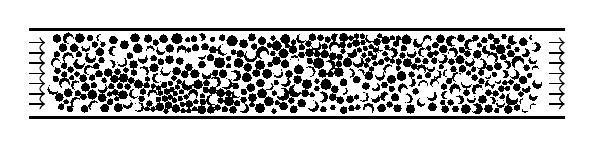
\begin{tikzpicture}[
  scale=2.0,
]

\foreach \y in {0.65,1.3,1.95,2.6,3.25,3.9,4.55}
  \draw[color=black,line width=0.5pt,solid,->]
    (0mm,\y mm) -- (1mm, \y mm);
% inlet arrows

\foreach \y in {0.65,1.3,1.95,2.6,3.25,3.9,4.55}
  \draw[color=black,line width=0.5pt,solid,->]
    (33mm,\y mm) -- (34mm, \y mm);
% outlet arrows

\filldraw[line width=0pt,black] (22.018465mm,1.7301593mm) circle (0.24716999mm);
\filldraw[line width=0pt,white] (21.93435mm,1.8316401mm) circle (0.17567399mm);

\filldraw[line width=0pt,black] (29.124408mm,2.435447mm) circle (0.1746042mm);
\filldraw[line width=0pt,white] (29.083648mm,2.5350955mm) circle (0.173219mm);

\filldraw[line width=0pt,black] (23.707936mm,1.656794mm) circle (0.28507471mm);
\filldraw[line width=0pt,white] (23.793675mm,1.5164935mm) circle (0.17567311mm);

\filldraw[line width=0pt,black] (30.009169mm,1.1604772mm) circle (0.17396896mm);
\filldraw[line width=0pt,white] (29.80313mm,1.3084506mm) circle (0.18255211mm);

\filldraw[line width=0pt,black] (31.336718mm,0.8095166mm) circle (0.17467739mm);
\filldraw[line width=0pt,white] (31.415026mm,0.7712897mm) circle (0.18210301mm);

\filldraw[line width=0pt,black] (29.38659mm,0.8786736mm) circle (0.21752247mm);
\filldraw[line width=0pt,white] (29.228719mm,0.8562496mm) circle (0.18169315mm);

\filldraw[line width=0pt,black] (22.004487mm,1.0006118mm) circle (0.2477091mm);
\filldraw[line width=0pt,white] (21.917763mm,1.172538mm) circle (0.17580636mm);

\filldraw[line width=0pt,black] (23.092122mm,3.9227006mm) circle (0.29039918mm);
\filldraw[line width=0pt,white] (22.943112mm,3.8760659mm) circle (0.17610235mm);

\filldraw[line width=0pt,black] (29.926432mm,0.6753806mm) circle (0.24690184mm);
\filldraw[line width=0pt,white] (29.937116mm,0.7885469mm) circle (0.18165982mm);

\filldraw[line width=0pt,black] (30.694065mm,4.7191788mm) circle (0.2876399mm);
\filldraw[line width=0pt,white] (30.911217mm,4.8104365mm) circle (0.18184472mm);

\filldraw[line width=0pt,black] (24.927755mm,2.885253mm) circle (0.26597986mm);
\filldraw[line width=0pt,white] (24.9042mm,2.7463421mm) circle (0.18182685mm);

\filldraw[line width=0pt,black] (26.497872mm,2.6163182mm) circle (0.21400233mm);
\filldraw[line width=0pt,white] (26.59039mm,2.5965486mm) circle (0.18170547mm);

\filldraw[line width=0pt,black] (31.996306mm,1.1298443mm) circle (0.2471246mm);
\filldraw[line width=0pt,white] (32.035366mm,1.3127973mm) circle (0.18167686mm);

\filldraw[line width=0pt,black] (22.571286mm,1.1499031mm) circle (0.26618084mm);
\filldraw[line width=0pt,white] (22.744498mm,1.0290525mm) circle (0.1752237mm);

\filldraw[line width=0pt,black] (28.44165mm,0.3616018mm) circle (0.3305877mm);
\filldraw[line width=0pt,white] (28.200489mm,0.387669mm) circle (0.1816057mm);

\filldraw[line width=0pt,black] (31.993264mm,0.4963167mm) circle (0.18206834mm);
\filldraw[line width=0pt,white] (32.043658mm,0.406665mm) circle (0.18037858mm);

\filldraw[line width=0pt,black] (31.902159mm,4.8806829mm) circle (0.13975493mm);
\filldraw[line width=0pt,white] (32.08199mm,4.9064077mm) circle (0.18208551mm);

\filldraw[line width=0pt,black] (26.913452mm,3.9392386mm) circle (0.28925837mm);
\filldraw[line width=0pt,white] (26.84047mm,3.8271296mm) circle (0.18204269mm);

\filldraw[line width=0pt,black] (22.307918mm,4.1898896mm) circle (0.17464248mm);
\filldraw[line width=0pt,white] (22.385207mm,4.2690084mm) circle (0.1757113mm);

\filldraw[line width=0pt,black] (27.334294mm,0.9339718mm) circle (0.25979744mm);
\filldraw[line width=0pt,white] (27.183329mm,0.9059348mm) circle (0.1812202mm);

\filldraw[line width=0pt,black] (24.681244mm,4.5396314mm) circle (0.28904875mm);
\filldraw[line width=0pt,white] (24.7899mm,4.6885016mm) circle (0.18190683mm);

\filldraw[line width=0pt,black] (24.292345mm,2.0249506mm) circle (0.23478403mm);
\filldraw[line width=0pt,white] (24.114789mm,2.0592106mm) circle (0.18225543mm);

\filldraw[line width=0pt,black] (25.910213mm,2.5358639mm) circle (0.2470511mm);
\filldraw[line width=0pt,white] (25.822798mm,2.6004331mm) circle (0.18209977mm);

\filldraw[line width=0pt,black] (32.264181mm,1.936298mm) circle (0.28883514mm);
\filldraw[line width=0pt,white] (32.333683mm,2.1146751mm) circle (0.18423974mm);

\filldraw[line width=0pt,black] (28.073239mm,0.9770611mm) circle (0.24687346mm);
\filldraw[line width=0pt,white] (28.067269mm,1.0957519mm) circle (0.18138278mm);

\filldraw[line width=0pt,black] (22.182286mm,3.74633mm) circle (0.17553306mm);
\filldraw[line width=0pt,white] (22.269067mm,3.717361mm) circle (0.17509431mm);

\filldraw[line width=0pt,black] (31.979358mm,3.4423801mm) circle (0.24696563mm);
\filldraw[line width=0pt,white] (32.023687mm,3.5657291mm) circle (0.18374441mm);

\filldraw[line width=0pt,black] (30.333856mm,3.1493168mm) circle (0.24793619mm);
\filldraw[line width=0pt,white] (30.184693mm,3.0973813mm) circle (0.18462372mm);

\filldraw[line width=0pt,black] (26.806863mm,4.6603721mm) circle (0.331423mm);
\filldraw[line width=0pt,white] (26.996148mm,4.6056694mm) circle (0.18203654mm);

\filldraw[line width=0pt,black] (32.123961mm,2.8969733mm) circle (0.18203333mm);
\filldraw[line width=0pt,white] (32.131597mm,2.7541232mm) circle (0.18292906mm);

\filldraw[line width=0pt,black] (24.883945mm,0.7783777mm) circle (0.25978623mm);
\filldraw[line width=0pt,white] (24.985039mm,0.8943296mm) circle (0.20656016mm);

\filldraw[line width=0pt,black] (25.270989mm,4.7682206mm) circle (0.26041393mm);
\filldraw[line width=0pt,white] (25.277793mm,4.6047199mm) circle (0.18205871mm);

\filldraw[line width=0pt,black] (31.482526mm,0.3058583mm) circle (0.17474411mm);
\filldraw[line width=0pt,white] (31.525579mm,0.4062538mm) circle (0.18097018mm);

\filldraw[line width=0pt,black] (32.156106mm,4.2799457mm) circle (0.28859635mm);
\filldraw[line width=0pt,white] (31.995829mm,4.282109mm) circle (0.18314262mm);

\filldraw[line width=0pt,black] (25.716075mm,2.0049081mm) circle (0.24712256mm);
\filldraw[line width=0pt,white] (25.80228mm,1.9062594mm) circle (0.18432663mm);

\filldraw[line width=0pt,black] (29.768694mm,2.1350637mm) circle (0.17499731mm);
\filldraw[line width=0pt,white] (29.724534mm,2.2618923mm) circle (0.18088896mm);

\filldraw[line width=0pt,black] (25.510362mm,2.9451469mm) circle (0.23490982mm);
\filldraw[line width=0pt,white] (25.481109mm,3.0748749mm) circle (0.18399191mm);

\filldraw[line width=0pt,black] (24.976013mm,3.956404mm) circle (0.26668077mm);
\filldraw[line width=0pt,white] (25.072502mm,3.9097023mm) circle (0.19092491mm);

\filldraw[line width=0pt,black] (31.51033mm,3.9020791mm) circle (0.24744348mm);
\filldraw[line width=0pt,white] (31.334211mm,4.0321131mm) circle (0.18175005mm);

\filldraw[line width=0pt,black] (27.974273mm,3.3335433mm) circle (0.27920779mm);
\filldraw[line width=0pt,white] (27.946218mm,3.4802341mm) circle (0.18322814mm);

\filldraw[line width=0pt,black] (26.264748mm,3.5284858mm) circle (0.28899843mm);
\filldraw[line width=0pt,white] (26.135264mm,3.6071689mm) circle (0.20451292mm);

\filldraw[line width=0pt,black] (30.185274mm,2.5620403mm) circle (0.24779083mm);
\filldraw[line width=0pt,white] (30.00573mm,2.5366669mm) circle (0.18406932mm);

\filldraw[line width=0pt,black] (26.438053mm,1.229725mm) circle (0.24701856mm);
\filldraw[line width=0pt,white] (26.554818mm,1.2119444mm) circle (0.18116416mm);

\filldraw[line width=0pt,black] (10.415059mm,1.3108756mm) circle (0.28903331mm);
\filldraw[line width=0pt,white] (10.3804mm,1.1276127mm) circle (0.19622074mm);

\filldraw[line width=0pt,black] (13.100491mm,2.4651385mm) circle (0.33129347mm);
\filldraw[line width=0pt,white] (12.924058mm,2.4471512mm) circle (0.22199639mm);

\filldraw[line width=0pt,black] (11.262098mm,2.5128799mm) circle (0.279099mm);
\filldraw[line width=0pt,white] (11.280203mm,2.69671mm) circle (0.22243512mm);

\filldraw[line width=0pt,black] (3.894523mm,3.595722mm) circle (0.33126317mm);
\filldraw[line width=0pt,white] (3.969473mm,3.7612523mm) circle (0.21901927mm);

\filldraw[line width=0pt,black] (7.688161mm,4.1092309mm) circle (0.23507219mm);
\filldraw[line width=0pt,white] (7.662345mm,3.9748682mm) circle (0.21265629mm);

\filldraw[line width=0pt,black] (27.031346mm,1.6005661mm) circle (0.33157145mm);
\filldraw[line width=0pt,white] (27.097806mm,1.4030988mm) circle (0.21919252mm);

\filldraw[line width=0pt,black] (24.279369mm,3.8861585mm) circle (0.28580681mm);
\filldraw[line width=0pt,white] (24.241288mm,4.0364174mm) circle (0.2080397mm);

\filldraw[line width=0pt,black] (13.66008mm,0.3783881mm) circle (0.2907061mm);
\filldraw[line width=0pt,white] (13.526674mm,0.4423918mm) circle (0.21358578mm);

\filldraw[line width=0pt,black] (8.651224mm,2.7357766mm) circle (0.28849554mm);
\filldraw[line width=0pt,white] (8.692073mm,2.8477584mm) circle (0.22387675mm);

\filldraw[line width=0pt,black] (6.644128mm,1.3133567mm) circle (0.28587947mm);
\filldraw[line width=0pt,white] (6.748793mm,1.367911mm) circle (0.22312223mm);

\filldraw[line width=0pt,black] (4.658632mm,1.6596094mm) circle (0.28921676mm);
\filldraw[line width=0pt,white] (4.588652mm,1.7855008mm) circle (0.22312223mm);

\filldraw[line width=0pt,black] (8.115328mm,2.3089573mm) circle (0.28937612mm);
\filldraw[line width=0pt,white] (8.225719mm,2.3064855mm) circle (0.2241929mm);

\filldraw[line width=0pt,black] (29.014059mm,4.106865mm) circle (0.24702712mm);
\filldraw[line width=0pt,white] (29.21619mm,4.2496541mm) circle (0.204766mm);

\filldraw[line width=0pt,black] (1.672317mm,3.2921164mm) circle (0.29010617mm);
\filldraw[line width=0pt,white] (1.745879mm,3.2141808mm) circle (0.2239569mm);

\filldraw[line width=0pt,black] (6.244382mm,0.6555685mm) circle (0.28819813mm);
\filldraw[line width=0pt,white] (6.187489mm,0.7977047mm) circle (0.2221482mm);

\filldraw[line width=0pt,black] (7.215603mm,3.5358008mm) circle (0.28533662mm);
\filldraw[line width=0pt,white] (7.170588mm,3.7322393mm) circle (0.21599931mm);

\filldraw[line width=0pt,black] (8.352453mm,4.046981mm) circle (0.26566778mm);
\filldraw[line width=0pt,white] (8.414166mm,4.2072075mm) circle (0.22385301mm);

\filldraw[line width=0pt,black] (2.479701mm,4.8309473mm) circle (0.33195603mm);
\filldraw[line width=0pt,white] (2.601933mm,4.7281144mm) circle (0.22325757mm);

\filldraw[line width=0pt,black] (30.823246mm,2.5280123mm) circle (0.2882202mm);
\filldraw[line width=0pt,white] (30.682935mm,2.6196908mm) circle (0.22400115mm);

\filldraw[line width=0pt,black] (24.037528mm,1.0072707mm) circle (0.28579621mm);
\filldraw[line width=0pt,white] (23.940916mm,0.9990744mm) circle (0.22371275mm);

\filldraw[line width=0pt,black] (15.238218mm,1.7901245mm) circle (0.2473843mm);
\filldraw[line width=0pt,white] (15.161849mm,1.8523325mm) circle (0.21299535mm);

\filldraw[line width=0pt,black] (13.124906mm,1.2812163mm) circle (0.24654318mm);
\filldraw[line width=0pt,white] (13.233761mm,1.3705567mm) circle (0.22240079mm);

\filldraw[line width=0pt,black] (5.20866mm,3.1887119mm) circle (0.24807166mm);
\filldraw[line width=0pt,white] (5.05391mm,3.1618588mm) circle (0.22298497mm);

\filldraw[line width=0pt,black] (9.680667mm,4.0842811mm) circle (0.2923003mm);
\filldraw[line width=0pt,white] (9.695245mm,3.8733686mm) circle (0.22254819mm);

\filldraw[line width=0pt,black] (3.767654mm,2.8326417mm) circle (0.28997354mm);
\filldraw[line width=0pt,white] (3.886299mm,2.7506464mm) circle (0.22402726mm);

\filldraw[line width=0pt,black] (5.908782mm,3.319853mm) circle (0.28867076mm);
\filldraw[line width=0pt,white] (5.854512mm,3.4018748mm) circle (0.22438293mm);

\filldraw[line width=0pt,black] (6.970174mm,0.45013mm) circle (0.29042451mm);
\filldraw[line width=0pt,white] (6.883719mm,0.4886236mm) circle (0.22297098mm);

\filldraw[line width=0pt,black] (10.961885mm,4.9234568mm) circle (0.21612495mm);
\filldraw[line width=0pt,white] (10.705554mm,4.8103305mm) circle (0.22286861mm);

\filldraw[line width=0pt,black] (3.158452mm,3.2091235mm) circle (0.32552104mm);
\filldraw[line width=0pt,white] (3.295mm,3.3726662mm) circle (0.22388319mm);

\filldraw[line width=0pt,black] (20.403439mm,2.6190501mm) circle (0.26066033mm);
\filldraw[line width=0pt,white] (20.273499mm,2.6264536mm) circle (0.22192861mm);

\filldraw[line width=0pt,black] (29.41273mm,3.6007975mm) circle (0.33107426mm);
\filldraw[line width=0pt,white] (29.331975mm,3.5147102mm) circle (0.24346543mm);

\filldraw[line width=0pt,black] (2.235046mm,1.9975052mm) circle (0.33355996mm);
\filldraw[line width=0pt,white] (2.286867mm,1.8635635mm) circle (0.22281676mm);

\filldraw[line width=0pt,black] (4.512105mm,4.8686373mm) circle (0.21559657mm);
\filldraw[line width=0pt,white] (4.631229mm,4.8489092mm) circle (0.22436251mm);

\filldraw[line width=0pt,black] (20.89458mm,3.3232724mm) circle (0.33224111mm);
\filldraw[line width=0pt,white] (20.826422mm,3.4532672mm) circle (0.23639354mm);

\filldraw[line width=0pt,black] (21.048364mm,2.6554972mm) circle (0.21559657mm);
\filldraw[line width=0pt,white] (20.954016mm,2.5180243mm) circle (0.23754789mm);

\filldraw[line width=0pt,black] (7.831719mm,1.2751766mm) circle (0.29477419mm);
\filldraw[line width=0pt,white] (7.863079mm,1.1557039mm) circle (0.22302849mm);

\filldraw[line width=0pt,black] (25.578431mm,1.1584686mm) circle (0.29013658mm);
\filldraw[line width=0pt,white] (25.478705mm,1.2750012mm) circle (0.22098688mm);

\filldraw[line width=0pt,black] (10.030765mm,1.8705106mm) circle (0.33231258mm);
\filldraw[line width=0pt,white] (10.13183mm,2.0798045mm) circle (0.22087721mm);

\filldraw[line width=0pt,black] (5.346621mm,4.035213mm) circle (0.2891104mm);
\filldraw[line width=0pt,white] (5.514901mm,3.9964664mm) circle (0.22375339mm);

\filldraw[line width=0pt,black] (10.951115mm,3.7072253mm) circle (0.21443321mm);
\filldraw[line width=0pt,white] (10.924273mm,3.8641274mm) circle (0.22331918mm);

\filldraw[line width=0pt,black] (21.24402mm,1.1131385mm) circle (0.29109639mm);
\filldraw[line width=0pt,white] (21.159401mm,1.1335494mm) circle (0.23763708mm);

\filldraw[line width=0pt,black] (3.587249mm,4.2619047mm) circle (0.25922106mm);
\filldraw[line width=0pt,white] (3.602677mm,4.4265346mm) circle (0.22282525mm);

\filldraw[line width=0pt,black] (22.269102mm,2.4632104mm) circle (0.28899028mm);
\filldraw[line width=0pt,white] (22.22738mm,2.6167371mm) circle (0.23352669mm);

\filldraw[line width=0pt,black] (16.868633mm,1.4935807mm) circle (0.37289799mm);
\filldraw[line width=0pt,white] (17.054018mm,1.6506659mm) circle (0.24353098mm);

\filldraw[line width=0pt,black] (2.948445mm,1.8601535mm) circle (0.27927813mm);
\filldraw[line width=0pt,white] (3.062364mm,1.781117mm) circle (0.22423411mm);

\filldraw[line width=0pt,black] (21.603878mm,4.8112528mm) circle (0.24763569mm);
\filldraw[line width=0pt,white] (21.701182mm,4.9078163mm) circle (0.23163427mm);

\filldraw[line width=0pt,black] (11.823175mm,2.0727241mm) circle (0.3268817mm);
\filldraw[line width=0pt,white] (11.678534mm,2.0047086mm) circle (0.25708831mm);

\filldraw[line width=0pt,black] (14.807191mm,3.9209061mm) circle (0.37385774mm);
\filldraw[line width=0pt,white] (14.900803mm,3.7729786mm) circle (0.23847523mm);

\filldraw[line width=0pt,black] (19.398615mm,4.8980679mm) circle (0.21809509mm);
\filldraw[line width=0pt,white] (19.728746mm,4.8056541mm) circle (0.23703024mm);

\filldraw[line width=0pt,black] (31.555874mm,1.6370187mm) circle (0.24732922mm);
\filldraw[line width=0pt,white] (31.460992mm,1.8895362mm) circle (0.23468077mm);

\filldraw[line width=0pt,black] (28.461687mm,1.5775827mm) circle (0.32541494mm);
\filldraw[line width=0pt,white] (28.573765mm,1.4444328mm) circle (0.23784943mm);

\filldraw[line width=0pt,black] (19.360491mm,4.2965536mm) circle (0.32535647mm);
\filldraw[line width=0pt,white] (19.406739mm,4.1610332mm) circle (0.23801402mm);

\filldraw[line width=0pt,black] (22.808094mm,2.8840792mm) circle (0.28891212mm);
\filldraw[line width=0pt,white] (22.902863mm,2.785604mm) circle (0.25054295mm);

\filldraw[line width=0pt,black] (17.266569mm,4.8148221mm) circle (0.29023988mm);
\filldraw[line width=0pt,white] (17.372891mm,4.9180386mm) circle (0.23755606mm);

\filldraw[line width=0pt,black] (20.509286mm,3.8831787mm) circle (0.29019461mm);
\filldraw[line width=0pt,white] (20.331816mm,4.1493179mm) circle (0.23718632mm);

\filldraw[line width=0pt,black] (18.235734mm,4.3582127mm) circle (0.29191212mm);
\filldraw[line width=0pt,white] (18.158778mm,4.461937mm) circle (0.23921238mm);

\filldraw[line width=0pt,black] (25.018296mm,1.876399mm) circle (0.28871963mm);
\filldraw[line width=0pt,white] (25.035928mm,1.7807957mm) circle (0.2475671mm);

\filldraw[line width=0pt,black] (19.104899mm,3.1280582mm) circle (0.32742941mm);
\filldraw[line width=0pt,white] (18.959051mm,3.072769mm) circle (0.23841616mm);

\filldraw[line width=0pt,black] (19.973444mm,1.4888208mm) circle (0.21481892mm);
\filldraw[line width=0pt,white] (19.851175mm,1.565216mm) circle (0.23741234mm);

\filldraw[line width=0pt,black] (21.546072mm,0.3835474mm) circle (0.33053298mm);
\filldraw[line width=0pt,white] (21.526909mm,0.2603021mm) circle (0.23701713mm);

\filldraw[line width=0pt,black] (27.965447mm,4.4347346mm) circle (0.32751297mm);
\filldraw[line width=0pt,white] (28.115158mm,4.3815549mm) circle (0.23509209mm);

\filldraw[line width=0pt,black] (16.277951mm,2.0516194mm) circle (0.28805887mm);
\filldraw[line width=0pt,white] (16.153805mm,2.1758288mm) circle (0.23696743mm);

\filldraw[line width=0pt,black] (31.026645mm,3.3045794mm) circle (0.37371137mm);
\filldraw[line width=0pt,white] (31.106328mm,3.1369906mm) circle (0.25722983mm);

\filldraw[line width=0pt,black] (16.849883mm,3.4961182mm) circle (0.24644783mm);
\filldraw[line width=0pt,white] (16.843903mm,3.3406326mm) circle (0.24160562mm);

\filldraw[line width=0pt,black] (18.631137mm,1.1061645mm) circle (0.33122788mm);
\filldraw[line width=0pt,white] (18.439412mm,1.1034406mm) circle (0.24411141mm);

\filldraw[line width=0pt,black] (28.692751mm,3.1945304mm) circle (0.33374148mm);
\filldraw[line width=0pt,white] (28.573153mm,3.2215995mm) circle (0.25033293mm);

\filldraw[line width=0pt,black] (12.545474mm,1.935869mm) circle (0.33243649mm);
\filldraw[line width=0pt,white] (12.445888mm,1.9926782mm) circle (0.25800352mm);

\filldraw[line width=0pt,black] (16.113202mm,1.2731645mm) circle (0.37358791mm);
\filldraw[line width=0pt,white] (15.949585mm,1.3869741mm) circle (0.2380485mm);

\filldraw[line width=0pt,black] (7.287332mm,2.7557982mm) circle (0.28633294mm);
\filldraw[line width=0pt,white] (7.166962mm,2.6567579mm) circle (0.25229848mm);

\filldraw[line width=0pt,black] (11.565929mm,0.9003942mm) circle (0.32515778mm);
\filldraw[line width=0pt,white] (11.70058mm,0.9459744mm) circle (0.27221628mm);

\filldraw[line width=0pt,black] (15.815287mm,2.6101946mm) circle (0.28786253mm);
\filldraw[line width=0pt,white] (15.750393mm,2.7207271mm) circle (0.24516455mm);

\filldraw[line width=0pt,black] (30.648525mm,0.9706596mm) circle (0.373598mm);
\filldraw[line width=0pt,white] (30.746713mm,1.1854326mm) circle (0.27286501mm);

\filldraw[line width=0pt,black] (2.461316mm,3.6174261mm) circle (0.32628081mm);
\filldraw[line width=0pt,white] (2.511106mm,3.4832046mm) circle (0.24435541mm);

\filldraw[line width=0pt,black] (18.037258mm,0.5220114mm) circle (0.33147232mm);
\filldraw[line width=0pt,white] (17.902103mm,0.6364536mm) circle (0.26785352mm);

\filldraw[line width=0pt,black] (17.818928mm,2.7274938mm) circle (0.33115316mm);
\filldraw[line width=0pt,white] (17.75414mm,2.6833067mm) circle (0.27287697mm);

\filldraw[line width=0pt,black] (4.117483mm,0.5360617mm) circle (0.33126939mm);
\filldraw[line width=0pt,white] (4.213404mm,0.4397749mm) circle (0.30447123mm);

\filldraw[line width=0pt,black] (2.962542mm,0.7616936mm) circle (0.32742543mm);
\filldraw[line width=0pt,white] (3.082649mm,0.6702032mm) circle (0.28759411mm);

\filldraw[line width=0pt,black] (12.29191mm,4.0899872mm) circle (0.3315287mm);
\filldraw[line width=0pt,white] (12.43768mm,4.169558mm) circle (0.28491934mm);

\filldraw[line width=0pt,black] (14.058245mm,3.7002904mm) circle (0.37295739mm);
\filldraw[line width=0pt,white] (14.076001mm,3.8338419mm) circle (0.29036651mm);

\filldraw[line width=0pt,black] (27.153079mm,2.3660073mm) circle (0.28983499mm);
\filldraw[line width=0pt,white] (27.248748mm,2.3119987mm) circle (0.25065634mm);

\filldraw[line width=0pt,black] (1.511951mm,1.5963025mm) circle (0.33090144mm);
\filldraw[line width=0pt,white] (1.57954mm,1.7308049mm) circle (0.30141652mm);

\filldraw[line width=0pt,black] (27.766425mm,1.9872761mm) circle (0.32503795mm);
\filldraw[line width=0pt,white] (27.794377mm,2.149862mm) circle (0.33508891mm);

\filldraw[line width=0pt,black] (29.249521mm,1.9010266mm) circle (0.29022486mm);
\filldraw[line width=0pt,white] (29.347307mm,2.075262mm) circle (0.1805231mm);

\filldraw[line width=0pt,white] (29.16919mm,1.6335076mm) circle (0.18171775mm);

\filldraw[line width=0pt,black] (10.132162mm,4.0931488mm) circle (0.13850288mm);
\filldraw[line width=0pt,black] (30.969474mm,4.1274072mm) circle (0.13908641mm);
\filldraw[line width=0pt,black] (30.444063mm,4.2913585mm) circle (0.13866492mm);
\filldraw[line width=0pt,black] (30.14856mm,4.9527324mm) circle (0.13939821mm);
\filldraw[line width=0pt,black] (21.259932mm,3.7576165mm) circle (0.13887385mm);
\filldraw[line width=0pt,black] (4.676123mm,4.4473972mm) circle (0.13874072mm);
\filldraw[line width=0pt,black] (8.94988mm,1.1012266mm) circle (0.13717489mm);
\filldraw[line width=0pt,black] (22.5929mm,3.8459084mm) circle (0.13785541mm);
\filldraw[line width=0pt,black] (8.674888mm,0.201377mm) circle (0.13905377mm);
\filldraw[line width=0pt,black] (14.143777mm,0.6118213mm) circle (0.13933866mm);
\filldraw[line width=0pt,black] (31.224078mm,1.2895281mm) circle (0.13886866mm);
\filldraw[line width=0pt,black] (15.487198mm,4.8442055mm) circle (0.13978215mm);
\filldraw[line width=0pt,black] (31.771043mm,2.4809153mm) circle (0.13963247mm);
\filldraw[line width=0pt,black] (9.40777mm,1.736749mm) circle (0.13883486mm);
\filldraw[line width=0pt,black] (9.770237mm,0.2365177mm) circle (0.13851263mm);
\filldraw[line width=0pt,black] (15.291087mm,3.166535mm) circle (0.13985378mm);
\filldraw[line width=0pt,black] (9.963742mm,1.1096327mm) circle (0.139531mm);
\filldraw[line width=0pt,black] (20.792104mm,1.1037774mm) circle (0.13884845mm);
\filldraw[line width=0pt,black] (24.789923mm,2.3812742mm) circle (0.13904318mm);
\filldraw[line width=0pt,black] (22.24938mm,4.9947966mm) circle (0.13915472mm);
\filldraw[line width=0pt,black] (27.901102mm,2.6268486mm) circle (0.13992071mm);
\filldraw[line width=0pt,black] (16.384172mm,4.3489007mm) circle (0.13858948mm);
\filldraw[line width=0pt,black] (19.927414mm,4.0145498mm) circle (0.13905697mm);
\filldraw[line width=0pt,black] (6.133579mm,2.8164537mm) circle (0.13918094mm);
\filldraw[line width=0pt,black] (7.864709mm,0.3344028mm) circle (0.13953435mm);
\filldraw[line width=0pt,black] (15.746136mm,0.743515mm) circle (0.13910904mm);
\filldraw[line width=0pt,black] (7.872138mm,1.7979244mm) circle (0.13890541mm);
\filldraw[line width=0pt,black] (15.540087mm,0.2021285mm) circle (0.13997894mm);
\filldraw[line width=0pt,black] (10.503964mm,0.348933mm) circle (0.13948045mm);
\filldraw[line width=0pt,black] (9.665134mm,1.437424mm) circle (0.13897064mm);
\filldraw[line width=0pt,black] (8.964672mm,1.9752671mm) circle (0.13826506mm);
\filldraw[line width=0pt,black] (10.063356mm,4.7419798mm) circle (0.13957932mm);
\filldraw[line width=0pt,black] (23.428188mm,2.9452357mm) circle (0.13903278mm);
\filldraw[line width=0pt,black] (21.650636mm,3.8707114mm) circle (0.13821651mm);
\filldraw[line width=0pt,black] (30.376882mm,1.6496325mm) circle (0.13876369mm);
\filldraw[line width=0pt,black] (9.729186mm,0.62528mm) circle (0.13702237mm);
\filldraw[line width=0pt,black] (23.061298mm,4.8612634mm) circle (0.13882079mm);
\filldraw[line width=0pt,black] (20.863424mm,0.4541594mm) circle (0.14019931mm);
\filldraw[line width=0pt,black] (20.958077mm,4.0872511mm) circle (0.1374433mm);
\filldraw[line width=0pt,black] (9.055093mm,1.5850561mm) circle (0.13888451mm);
\filldraw[line width=0pt,black] (11.641671mm,4.7642992mm) circle (0.1398072mm);
\filldraw[line width=0pt,black] (22.717519mm,3.5208726mm) circle (0.13908528mm);
\filldraw[line width=0pt,black] (8.332031mm,1.3492658mm) circle (0.13822887mm);
\filldraw[line width=0pt,black] (18.267159mm,1.6438743mm) circle (0.1394827mm);
\filldraw[line width=0pt,black] (20.420929mm,4.845512mm) circle (0.13885282mm);
\filldraw[line width=0pt,black] (19.2821mm,0.429216mm) circle (0.13947596mm);
\filldraw[line width=0pt,black] (21.189264mm,4.5690769mm) circle (0.1375947mm);
\filldraw[line width=0pt,black] (28.225031mm,2.8645929mm) circle (0.13940884mm);
\filldraw[line width=0pt,black] (12.660696mm,3.0865035mm) circle (0.13911386mm);
\filldraw[line width=0pt,black] (3.027663mm,2.5658623mm) circle (0.13973693mm);
\filldraw[line width=0pt,black] (15.2455mm,4.3875433mm) circle (0.13955092mm);
\filldraw[line width=0pt,black] (21.868004mm,3.6080242mm) circle (0.13842899mm);
\filldraw[line width=0pt,black] (12.967269mm,3.9467992mm) circle (0.13935437mm);
\filldraw[line width=0pt,black] (30.201523mm,2.0109952mm) circle (0.13833368mm);
\filldraw[line width=0pt,black] (25.824675mm,3.9003958mm) circle (0.13946036mm);
\filldraw[line width=0pt,black] (9.274736mm,1.3214113mm) circle (0.13898338mm);
\filldraw[line width=0pt,black] (21.95796mm,3.2181852mm) circle (0.13891933mm);
\filldraw[line width=0pt,black] (21.975109mm,4.0922893mm) circle (0.13832407mm);
\filldraw[line width=0pt,black] (12.655784mm,3.5517194mm) circle (0.13784076mm);
\filldraw[line width=0pt,black] (10.995816mm,1.1796195mm) circle (0.13946827mm);
\filldraw[line width=0pt,black] (26.167414mm,3.0309016mm) circle (0.13957932mm);
\filldraw[line width=0pt,black] (23.054766mm,3.3944572mm) circle (0.13966704mm);
\filldraw[line width=0pt,black] (10.58113mm,0.8005183mm) circle (0.13918194mm);
\filldraw[line width=0pt,black] (21.341521mm,4.1903308mm) circle (0.13880661mm);
\filldraw[line width=0pt,black] (30.583859mm,2.0508043mm) circle (0.13820135mm);
\filldraw[line width=0pt,black] (26.24731mm,0.751561mm) circle (0.13902785mm);
\filldraw[line width=0pt,black] (2.698244mm,2.3272574mm) circle (0.13896806mm);
\filldraw[line width=0pt,black] (29.68868mm,0.242872mm) circle (0.13919093mm);
\filldraw[line width=0pt,black] (20.781365mm,4.9687994mm) circle (0.13730916mm);
\filldraw[line width=0pt,black] (16.782393mm,4.5823074mm) circle (0.13856971mm);
\filldraw[line width=0pt,black] (28.580833mm,4.4033335mm) circle (0.13888821mm);
\filldraw[line width=0pt,black] (21.51524mm,3.456316mm) circle (0.13760099mm);
\filldraw[line width=0pt,black] (4.75741mm,2.1681228mm) circle (0.14010593mm);
\filldraw[line width=0pt,black] (9.214564mm,0.9012291mm) circle (0.13910975mm);
\filldraw[line width=0pt,black] (7.49626mm,2.2510825mm) circle (0.13905659mm);
\filldraw[line width=0pt,black] (18.261335mm,2.1102405mm) circle (0.13911007mm);
\filldraw[line width=0pt,black] (20.341497mm,4.3931356mm) circle (0.13850707mm);
\filldraw[line width=0pt,black] (7.481159mm,0.3510657mm) circle (0.13811751mm);
\filldraw[line width=0pt,black] (9.52004mm,2.0740332mm) circle (0.1392547mm);
\filldraw[line width=0pt,black] (23.43997mm,4.8413581mm) circle (0.13766145mm);
\filldraw[line width=0pt,black] (5.101877mm,1.2947471mm) circle (0.13952329mm);
\filldraw[line width=0pt,black] (21.735784mm,2.8830671mm) circle (0.13922453mm);
\filldraw[line width=0pt,black] (22.716201mm,4.2534265mm) circle (0.13834837mm);
\filldraw[line width=0pt,black] (29.534671mm,2.5453591mm) circle (0.1389823mm);
\filldraw[line width=0pt,black] (21.400171mm,3.1231763mm) circle (0.13889961mm);
\filldraw[line width=0pt,black] (15.559736mm,1.3448287mm) circle (0.13816319mm);
\filldraw[line width=0pt,black] (9.186667mm,2.3110442mm) circle (0.13975493mm);
\filldraw[line width=0pt,black] (9.585112mm,1.004652mm) circle (0.13785659mm);
\filldraw[line width=0pt,black] (21.154137mm,4.9600672mm) circle (0.13878263mm);
\filldraw[line width=0pt,black] (15.681852mm,2.0193019mm) circle (0.13939206mm);
\filldraw[line width=0pt,black] (21.710525mm,4.2967538mm) circle (0.13900826mm);
\filldraw[line width=0pt,black] (15.470186mm,3.8726582mm) circle (0.1399396mm);
\filldraw[line width=0pt,black] (5.557064mm,0.984788mm) circle (0.13856983mm);
\filldraw[line width=0pt,black] (2.340986mm,0.7942823mm) circle (0.13867249mm);
\filldraw[line width=0pt,black] (10.137902mm,0.2284164mm) circle (0.13801506mm);
\filldraw[line width=0pt,black] (17.956522mm,1.2474799mm) circle (0.13821955mm);
\filldraw[line width=0pt,black] (8.205326mm,0.9437805mm) circle (0.13919506mm);
\filldraw[line width=0pt,black] (8.206317mm,1.6734685mm) circle (0.13856183mm);
\filldraw[line width=0pt,black] (22.889491mm,0.6370575mm) circle (0.17558734mm);
\filldraw[line width=0pt,black] (23.018951mm,1.621364mm) circle (0.17491109mm);
\filldraw[line width=0pt,black] (24.669577mm,3.432819mm) circle (0.17408219mm);
\filldraw[line width=0pt,black] (4.254197mm,3.0684182mm) circle (0.17532075mm);
\filldraw[line width=0pt,black] (23.783605mm,4.2099249mm) circle (0.17554328mm);
\filldraw[line width=0pt,black] (29.316573mm,4.9471436mm) circle (0.17542089mm);
\filldraw[line width=0pt,black] (10.460252mm,4.8010144mm) circle (0.17514822mm);
\filldraw[line width=0pt,black] (26.667557mm,2.1263378mm) circle (0.1742936mm);
\filldraw[line width=0pt,black] (18.766931mm,4.3177115mm) circle (0.17352706mm);
\filldraw[line width=0pt,black] (19.666447mm,3.2100202mm) circle (0.1747019mm);
\filldraw[line width=0pt,black] (20.465058mm,0.3932838mm) circle (0.17507576mm);
\filldraw[line width=0pt,black] (27.761746mm,1.3794262mm) circle (0.17614856mm);
\filldraw[line width=0pt,black] (13.631287mm,1.4239174mm) circle (0.17441716mm);
\filldraw[line width=0pt,black] (13.61728mm,0.9211878mm) circle (0.17359229mm);
\filldraw[line width=0pt,black] (3.989987mm,2.3288263mm) circle (0.17453846mm);
\filldraw[line width=0pt,black] (2.221851mm,2.5388106mm) circle (0.17318612mm);
\filldraw[line width=0pt,black] (5.598661mm,2.70456mm) circle (0.17539442mm);
\filldraw[line width=0pt,black] (28.712823mm,2.1044988mm) circle (0.17424651mm);
\filldraw[line width=0pt,black] (29.667097mm,4.6605861mm) circle (0.17588718mm);
\filldraw[line width=0pt,black] (12.15885mm,0.878742mm) circle (0.1743269mm);
\filldraw[line width=0pt,black] (29.238444mm,2.9450103mm) circle (0.17523994mm);
\filldraw[line width=0pt,black] (6.254025mm,1.7632059mm) circle (0.17510883mm);
\filldraw[line width=0pt,black] (26.935087mm,2.8699581mm) circle (0.1762201mm);
\filldraw[line width=0pt,black] (14.280337mm,4.3156072mm) circle (0.17526761mm);
\filldraw[line width=0pt,black] (3.859922mm,4.8560187mm) circle (0.17491105mm);
\filldraw[line width=0pt,black] (4.167217mm,4.438767mm) circle (0.17491078mm);
\filldraw[line width=0pt,black] (12.246212mm,4.8650841mm) circle (0.17549973mm);
\filldraw[line width=0pt,black] (28.699509mm,2.6540052mm) circle (0.17318668mm);
\filldraw[line width=0pt,black] (29.442422mm,4.2821948mm) circle (0.17391974mm);
\filldraw[line width=0pt,black] (7.139541mm,0.9856667mm) circle (0.17488147mm);
\filldraw[line width=0pt,black] (30.978341mm,0.4294684mm) circle (0.174816mm);
\filldraw[line width=0pt,black] (26.816909mm,3.3447432mm) circle (0.17567443mm);
\filldraw[line width=0pt,black] (28.288581mm,2.3441313mm) circle (0.17490752mm);
\filldraw[line width=0pt,black] (17.727532mm,4.4905948mm) circle (0.17455327mm);
\filldraw[line width=0pt,black] (28.338436mm,4.8527676mm) circle (0.17401682mm);
\filldraw[line width=0pt,black] (25.368926mm,4.2109262mm) circle (0.13908688mm);
\filldraw[line width=0pt,black] (17.306441mm,4.2695616mm) circle (0.17427324mm);
\filldraw[line width=0pt,black] (17.294135mm,3.7734958mm) circle (0.17477889mm);
\filldraw[line width=0pt,black] (2.583863mm,0.3427276mm) circle (0.17511243mm);
\filldraw[line width=0pt,black] (19.120074mm,2.5614586mm) circle (0.17390165mm);
\filldraw[line width=0pt,black] (17.814921mm,3.395546mm) circle (0.17566194mm);
\filldraw[line width=0pt,black] (2.635886mm,2.8493534mm) circle (0.17543144mm);
\filldraw[line width=0pt,black] (5.761396mm,1.8137727mm) circle (0.1738548mm);
\filldraw[line width=0pt,black] (1.758605mm,3.8231958mm) circle (0.17510007mm);
\filldraw[line width=0pt,black] (18.95671mm,4.7541437mm) circle (0.17484878mm);
\filldraw[line width=0pt,black] (23.293093mm,4.4929188mm) circle (0.17580805mm);
\filldraw[line width=0pt,black] (25.163686mm,3.3770389mm) circle (0.17446457mm);
\filldraw[line width=0pt,black] (11.208832mm,1.5505969mm) circle (0.17399605mm);
\filldraw[line width=0pt,black] (1.799736mm,2.7608876mm) circle (0.17526452mm);
\filldraw[line width=0pt,black] (26.333912mm,1.7579594mm) circle (0.17556223mm);
\filldraw[line width=0pt,black] (2.022174mm,0.4858362mm) circle (0.17501076mm);
\filldraw[line width=0pt,black] (1.687421mm,2.2490529mm) circle (0.17523994mm);
\filldraw[line width=0pt,black] (30.100719mm,3.6330307mm) circle (0.17564983mm);
\filldraw[line width=0pt,black] (29.972827mm,1.6285622mm) circle (0.17479372mm);
\filldraw[line width=0pt,black] (3.157987mm,3.8143391mm) circle (0.1747423mm);
\filldraw[line width=0pt,black] (27.8352mm,3.8513789mm) circle (0.17535756mm);
\filldraw[line width=0pt,black] (22.351742mm,3.3236497mm) circle (0.17239025mm);
\filldraw[line width=0pt,black] (26.759592mm,0.7584411mm) circle (0.17460908mm);
\filldraw[line width=0pt,black] (23.699647mm,3.7495445mm) circle (0.17565564mm);
\filldraw[line width=0pt,black] (13.109305mm,1.8004901mm) circle (0.17600995mm);
\filldraw[line width=0pt,black] (28.899223mm,4.706869mm) circle (0.17367488mm);
\filldraw[line width=0pt,black] (23.465632mm,3.3417941mm) circle (0.17475891mm);
\filldraw[line width=0pt,black] (13.197949mm,0.7082358mm) circle (0.17516971mm);
\filldraw[line width=0pt,black] (29.61282mm,1.3311788mm) circle (0.17510609mm);
\filldraw[line width=0pt,black] (25.713998mm,3.4094085mm) circle (0.17502913mm);
\filldraw[line width=0pt,black] (6.392401mm,3.7292783mm) circle (0.18249307mm);
\filldraw[line width=0pt,black] (5.210615mm,1.787221mm) circle (0.17440379mm);
\filldraw[line width=0pt,black] (5.139389mm,0.7966891mm) circle (0.17530715mm);
\filldraw[line width=0pt,black] (24.530531mm,1.4633757mm) circle (0.18210301mm);
\filldraw[line width=0pt,black] (6.647252mm,2.6607027mm) circle (0.17479514mm);
\filldraw[line width=0pt,black] (7.905157mm,3.5714189mm) circle (0.17455416mm);
\filldraw[line width=0pt,black] (24.276618mm,2.5339094mm) circle (0.17488714mm);
\filldraw[line width=0pt,black] (18.275326mm,3.8418616mm) circle (0.17333081mm);
\filldraw[line width=0pt,black] (24.448319mm,3.0422243mm) circle (0.18309185mm);
\filldraw[line width=0pt,black] (3.450614mm,1.1106478mm) circle (0.17550245mm);
\filldraw[line width=0pt,black] (31.584697mm,2.9612993mm) circle (0.17494434mm);
\filldraw[line width=0pt,black] (27.061443mm,0.3402689mm) circle (0.17607037mm);
\filldraw[line width=0pt,black] (4.106395mm,1.8505363mm) circle (0.17523956mm);
\filldraw[line width=0pt,black] (12.421098mm,0.3335246mm) circle (0.17466936mm);
\filldraw[line width=0pt,black] (18.501632mm,4.8632753mm) circle (0.17411561mm);
\filldraw[line width=0pt,black] (16.645866mm,0.8790408mm) circle (0.17630428mm);
\filldraw[line width=0pt,black] (5.458788mm,1.4021157mm) circle (0.1828399mm);
\filldraw[line width=0pt,black] (11.258305mm,1.9894487mm) circle (0.17433695mm);
\filldraw[line width=0pt,black] (6.477299mm,2.1570656mm) circle (0.18335831mm);
\filldraw[line width=0pt,black] (12.649395mm,1.3538097mm) circle (0.17502564mm);
\filldraw[line width=0pt,black] (8.613054mm,1.0048896mm) circle (0.17577797mm);
\filldraw[line width=0pt,black] (18.673852mm,0.3273102mm) circle (0.17647966mm);
\filldraw[line width=0pt,black] (7.630014mm,0.7011365mm) circle (0.17532253mm);
\filldraw[line width=0pt,black] (29.16195mm,1.3716323mm) circle (0.17399637mm);
\filldraw[line width=0pt,black] (8.035363mm,4.5619476mm) circle (0.17623652mm);
\filldraw[line width=0pt,black] (25.466409mm,3.7945627mm) circle (0.18148102mm);
\filldraw[line width=0pt,black] (11.800508mm,2.6357095mm) circle (0.17480573mm);
\filldraw[line width=0pt,black] (11.964952mm,0.4432117mm) circle (0.17585349mm);
\filldraw[line width=0pt,black] (7.224775mm,1.4473692mm) circle (0.17644218mm);
\filldraw[line width=0pt,black] (25.784834mm,4.4007803mm) circle (0.17598471mm);
\filldraw[line width=0pt,black] (25.327849mm,2.4950872mm) circle (0.17566335mm);
\filldraw[line width=0pt,black] (7.458653mm,1.8493506mm) circle (0.175047mm);
\filldraw[line width=0pt,black] (11.024815mm,0.791497mm) circle (0.17350076mm);
\filldraw[line width=0pt,black] (27.473379mm,4.0862521mm) circle (0.17516873mm);
\filldraw[line width=0pt,black] (3.092924mm,1.3441548mm) circle (0.17609467mm);
\filldraw[line width=0pt,black] (19.896484mm,4.4053398mm) circle (0.17369111mm);
\filldraw[line width=0pt,black] (2.213668mm,3.0893111mm) circle (0.17478473mm);
\filldraw[line width=0pt,black] (22.560492mm,1.8607285mm) circle (0.18226823mm);
\filldraw[line width=0pt,black] (19.711003mm,3.6443482mm) circle (0.17413062mm);
\filldraw[line width=0pt,black] (19.961547mm,2.0316034mm) circle (0.2142307mm);
\filldraw[line width=0pt,black] (8.362102mm,3.3372199mm) circle (0.18397895mm);
\filldraw[line width=0pt,black] (8.738781mm,1.4476422mm) circle (0.1757412mm);
\filldraw[line width=0pt,black] (8.570044mm,1.8707473mm) circle (0.17358184mm);
\filldraw[line width=0pt,black] (11.651572mm,1.5154609mm) circle (0.21785853mm);
\filldraw[line width=0pt,black] (4.589712mm,3.4423322mm) circle (0.17671448mm);
\filldraw[line width=0pt,black] (11.170973mm,4.2970547mm) circle (0.21316873mm);
\filldraw[line width=0pt,black] (27.414554mm,4.8402532mm) circle (0.21656255mm);
\filldraw[line width=0pt,black] (30.581854mm,3.8574431mm) circle (0.21700602mm);
\filldraw[line width=0pt,black] (27.508392mm,2.8935159mm) circle (0.21737131mm);
\filldraw[line width=0pt,black] (20.371213mm,0.952242mm) circle (0.21477081mm);
\filldraw[line width=0pt,black] (12.942633mm,0.2970527mm) circle (0.2169377mm);
\filldraw[line width=0pt,black] (14.425632mm,2.622341mm) circle (0.21864248mm);
\filldraw[line width=0pt,black] (16.497239mm,2.5748486mm) circle (0.21859289mm);
\filldraw[line width=0pt,black] (19.264803mm,1.0919207mm) circle (0.21433702mm);
\filldraw[line width=0pt,black] (10.158045mm,0.6622071mm) circle (0.21414578mm);
\filldraw[line width=0pt,black] (11.515919mm,3.5980183mm) circle (0.21383847mm);
\filldraw[line width=0pt,black] (3.511021mm,0.3537352mm) circle (0.21776845mm);
\filldraw[line width=0pt,black] (10.552164mm,4.2423369mm) circle (0.21484002mm);
\filldraw[line width=0pt,black] (29.758107mm,3.0500582mm) circle (0.21748506mm);
\filldraw[line width=0pt,black] (3.416355mm,2.3008143mm) circle (0.2174623mm);
\filldraw[line width=0pt,black] (17.515155mm,1.3425991mm) circle (0.21797181mm);
\filldraw[line width=0pt,black] (19.405118mm,1.5982511mm) circle (0.21383519mm);
\filldraw[line width=0pt,black] (30.955471mm,1.7243097mm) circle (0.21798068mm);
\filldraw[line width=0pt,black] (10.962214mm,3.1637241mm) circle (0.21538085mm);
\filldraw[line width=0pt,black] (19.751576mm,0.8981977mm) circle (0.21291203mm);
\filldraw[line width=0pt,black] (10.133518mm,2.9912825mm) circle (0.21292718mm);
\filldraw[line width=0pt,black] (20.791613mm,2.2052198mm) circle (0.21320368mm);
\filldraw[line width=0pt,black] (9.877854mm,2.5424606mm) circle (0.2135771mm);
\filldraw[line width=0pt,black] (26.412947mm,0.3292892mm) circle (0.21418574mm);
\filldraw[line width=0pt,black] (21.373565mm,1.7983864mm) circle (0.21401727mm);
\filldraw[line width=0pt,black] (11.657232mm,4.1058202mm) circle (0.21247562mm);
\filldraw[line width=0pt,black] (4.425596mm,2.5819277mm) circle (0.21346965mm);
\filldraw[line width=0pt,black] (9.548803mm,3.3950386mm) circle (0.21475903mm);
\filldraw[line width=0pt,black] (19.962446mm,0.2723994mm) circle (0.21425082mm);
\filldraw[line width=0pt,black] (8.842779mm,0.5944217mm) circle (0.21572621mm);
\filldraw[line width=0pt,black] (22.080896mm,4.5990826mm) circle (0.21610437mm);
\filldraw[line width=0pt,black] (11.528839mm,0.2999721mm) circle (0.21853152mm);
\filldraw[line width=0pt,black] (13.407378mm,3.8520661mm) circle (0.21670932mm);
\filldraw[line width=0pt,black] (16.787215mm,0.3107269mm) circle (0.2192761mm);
\filldraw[line width=0pt,black] (20.766088mm,4.5340972mm) circle (0.21332114mm);
\filldraw[line width=0pt,black] (30.413971mm,0.3167156mm) circle (0.24681055mm);
\filldraw[line width=0pt,black] (17.982835mm,4.8981297mm) circle (0.21614443mm);
\filldraw[line width=0pt,black] (5.330605mm,4.7211111mm) circle (0.2469893mm);
\filldraw[line width=0pt,black] (14.138609mm,4.8819512mm) circle (0.21723132mm);
\filldraw[line width=0pt,black] (26.119223mm,4.7949161mm) circle (0.24668401mm);
\filldraw[line width=0pt,black] (28.782958mm,0.9544964mm) circle (0.24645681mm);
\filldraw[line width=0pt,black] (2.85027mm,4.2202876mm) circle (0.24735451mm);
\filldraw[line width=0pt,black] (31.356957mm,2.1841281mm) circle (0.2467572mm);
\filldraw[line width=0pt,black] (1.755281mm,4.8337136mm) circle (0.24671681mm);
\filldraw[line width=0pt,black] (13.880037mm,2.9887861mm) circle (0.24676821mm);
\filldraw[line width=0pt,black] (14.678531mm,1.9900342mm) circle (0.24708258mm);
\filldraw[line width=0pt,black] (23.378238mm,0.3851702mm) circle (0.23493063mm);
\filldraw[line width=0pt,black] (5.014255mm,2.658447mm) circle (0.24610988mm);
\filldraw[line width=0pt,black] (23.232451mm,1.0855023mm) circle (0.23498822mm);
\filldraw[line width=0pt,black] (19.274463mm,3.6814639mm) circle (0.21741215mm);
\filldraw[line width=0pt,black] (22.388903mm,0.4018195mm) circle (0.24662507mm);
\filldraw[line width=0pt,black] (17.799368mm,3.9166968mm) circle (0.2474079mm);
\filldraw[line width=0pt,black] (28.454802mm,3.8207983mm) circle (0.24656287mm);
\filldraw[line width=0pt,black] (16.747954mm,4.1276688mm) circle (0.24680967mm);
\filldraw[line width=0pt,black] (7.54465mm,4.8104107mm) circle (0.23478091mm);
\filldraw[line width=0pt,black] (31.363568mm,4.6026365mm) circle (0.24683236mm);
\filldraw[line width=0pt,black] (25.594005mm,0.4733169mm) circle (0.24732951mm);
\filldraw[line width=0pt,black] (8.922352mm,4.1967825mm) circle (0.24732951mm);
\filldraw[line width=0pt,black] (14.778004mm,4.667525mm) circle (0.24704512mm);
\filldraw[line width=0pt,black] (4.485629mm,3.9647934mm) circle (0.24740011mm);
\filldraw[line width=0pt,black] (16.245979mm,3.2050848mm) circle (0.24686966mm);
\filldraw[line width=0pt,black] (6.042267mm,4.4166322mm) circle (0.25946094mm);
\filldraw[line width=0pt,black] (9.316687mm,0.3802254mm) circle (0.2465239mm);
\filldraw[line width=0pt,black] (18.620745mm,2.6064156mm) circle (0.24699847mm);
\filldraw[line width=0pt,black] (5.41298mm,2.24886mm) circle (0.23397229mm);
\filldraw[line width=0pt,black] (29.167968mm,0.3595698mm) circle (0.24721134mm);
\filldraw[line width=0pt,black] (8.535077mm,4.7940188mm) circle (0.24733172mm);
\filldraw[line width=0pt,black] (8.906492mm,3.4677487mm) circle (0.24703425mm);
\filldraw[line width=0pt,black] (4.628403mm,1.054834mm) circle (0.24640136mm);
\filldraw[line width=0pt,black] (17.046463mm,2.209544mm) circle (0.24687321mm);
\filldraw[line width=0pt,black] (22.632004mm,4.7141401mm) circle (0.24689079mm);
\filldraw[line width=0pt,black] (18.76593mm,3.8287679mm) circle (0.24754639mm);
\filldraw[line width=0pt,black] (6.626389mm,3.1695614mm) circle (0.23543112mm);
\filldraw[line width=0pt,black] (8.295639mm,0.4810489mm) circle (0.24763206mm);
\filldraw[line width=0pt,black] (2.468101mm,1.3771485mm) circle (0.24680326mm);
\filldraw[line width=0pt,black] (7.924591mm,2.961275mm) circle (0.25922212mm);
\filldraw[line width=0pt,black] (9.357122mm,2.7478055mm) circle (0.24734794mm);
\filldraw[line width=0pt,black] (2.142291mm,4.2388691mm) circle (0.24643292mm);
\filldraw[line width=0pt,black] (1.911025mm,1.0895914mm) circle (0.24744863mm);
\filldraw[line width=0pt,black] (15.685116mm,3.4060571mm) circle (0.24761746mm);
\filldraw[line width=0pt,black] (14.174729mm,1.0675016mm) circle (0.24646037mm);
\filldraw[line width=0pt,black] (6.716867mm,4.8566123mm) circle (0.2661956mm);
\filldraw[line width=0pt,black] (12.158461mm,1.366622mm) circle (0.24682972mm);
\filldraw[line width=0pt,black] (19.966646mm,4.8975543mm) circle (0.26038915mm);
\filldraw[line width=0pt,black] (14.073728mm,1.7034044mm) circle (0.24892981mm);
\filldraw[line width=0pt,black] (6.927002mm,1.9216103mm) circle (0.26032669mm);
\filldraw[line width=0pt,black] (13.617877mm,4.4839075mm) circle (0.24671688mm);
\filldraw[line width=0pt,black] (23.00056mm,2.2343434mm) circle (0.26033303mm);
\filldraw[line width=0pt,black] (24.207682mm,0.3382524mm) circle (0.26618786mm);
\filldraw[line width=0pt,black] (5.652679mm,0.4276572mm) circle (0.25955227mm);
\filldraw[line width=0pt,black] (12.302011mm,2.5866863mm) circle (0.24707293mm);
\filldraw[line width=0pt,black] (27.35233mm,3.4675956mm) circle (0.26043776mm);
\filldraw[line width=0pt,black] (5.951667mm,1.2380745mm) circle (0.26684002mm);
\filldraw[line width=0pt,black] (3.570883mm,1.7283177mm) circle (0.26024755mm);
\filldraw[line width=0pt,black] (10.956286mm,0.2967567mm) circle (0.26033222mm);
\filldraw[line width=0pt,black] (23.99924mm,3.2740001mm) circle (0.26012842mm);
\filldraw[line width=0pt,black] (21.56488mm,2.4475207mm) circle (0.2491525mm);
\filldraw[line width=0pt,black] (14.650236mm,3.1414523mm) circle (0.2890177mm);
\filldraw[line width=0pt,black] (17.303424mm,0.7116232mm) circle (0.24785604mm);
\filldraw[line width=0pt,black] (4.804021mm,0.4010925mm) circle (0.24896132mm);
\filldraw[line width=0pt,black] (26.297828mm,4.1433281mm) circle (0.24865363mm);
\filldraw[line width=0pt,black] (10.519229mm,2.5740279mm) circle (0.2603643mm);
\filldraw[line width=0pt,black] (10.718068mm,1.9001681mm) circle (0.2789229mm);
\filldraw[line width=0pt,black] (16.148622mm,0.5281677mm) circle (0.24714923mm);
\filldraw[line width=0pt,black] (5.992685mm,2.3086504mm) circle (0.26625675mm);
\filldraw[line width=0pt,black] (6.886977mm,4.1908218mm) circle (0.28587166mm);
\filldraw[line width=0pt,black] (15.109778mm,2.5858049mm) circle (0.28770256mm);
\filldraw[line width=0pt,black] (17.634108mm,1.9148135mm) circle (0.28766564mm);
\filldraw[line width=0pt,black] (20.207204mm,3.2977939mm) circle (0.27968399mm);
\filldraw[line width=0pt,black] (16.144202mm,3.8707327mm) circle (0.28878671mm);
\filldraw[line width=0pt,black] (13.812802mm,2.3469382mm) circle (0.28786253mm);
\filldraw[line width=0pt,black] (15.212352mm,0.8295496mm) circle (0.2878563mm);
\filldraw[line width=0pt,black] (29.930266mm,4.132884mm) circle (0.28997462mm);
\filldraw[line width=0pt,black] (23.637639mm,2.443873mm) circle (0.28512987mm);
\filldraw[line width=0pt,black] (14.783037mm,1.325871mm) circle (0.28818284mm);
\filldraw[line width=0pt,black] (17.109957mm,2.8470105mm) circle (0.28794473mm);
\filldraw[line width=0pt,black] (27.720608mm,0.3450498mm) circle (0.2793249mm);
\filldraw[line width=0pt,black] (14.656618mm,0.39787mm) circle (0.28526852mm);
\filldraw[line width=0pt,black] (4.009092mm,1.2557625mm) circle (0.29003474mm);
\filldraw[line width=0pt,black] (19.65937mm,2.6825762mm) circle (0.28040455mm);
\filldraw[line width=0pt,black] (23.952617mm,4.7473228mm) circle (0.28982837mm);
\filldraw[line width=0pt,black] (13.291079mm,3.2793578mm) circle (0.28938832mm);
\filldraw[line width=0pt,black] (15.709568mm,4.3614989mm) circle (0.29309839mm);
\filldraw[line width=0pt,black] (3.204252mm,4.8506075mm) circle (0.27976181mm);
\filldraw[line width=0pt,black] (16.265575mm,4.7955098mm) circle (0.28747191mm);
\filldraw[line width=0pt,black] (12.690258mm,0.8388729mm) circle (0.29091339mm);
\filldraw[line width=0pt,black] (12.079982mm,3.2798108mm) circle (0.33097683mm);
\filldraw[line width=0pt,black] (9.376923mm,4.8109774mm) circle (0.33106905mm);
\filldraw[line width=0pt,black] (12.883138mm,4.6710712mm) circle (0.33125419mm);
\filldraw[line width=0pt,black] (18.843142mm,1.9161669mm) circle (0.33117956mm);
\filldraw[line width=0pt,black] (18.379338mm,3.2594754mm) circle (0.33286547mm);
\draw[line width=0.4mm] (0mm,-0.2mm) -- (34mm,-0.2mm);
\draw[line width=0.4mm] (0mm,5.4mm) -- (34mm,5.4mm);
% outer walls


\end{tikzpicture}

\else
  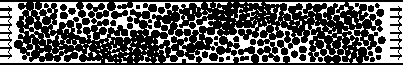
\includegraphics{circleGrains.pdf}
  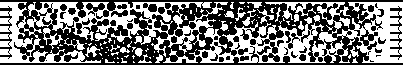
\includegraphics{beanGrains.pdf}
\fi
\caption{\label{f:beans} These geometry, which we call the {\em circle
geometry} and the {\em bean geometry}, consist of 465 exclusions and
has a porosity (the ratio of the region that contains the fluid) of
0.46 ({\em circle}) and 0. ({\em bean}).  The outer wall is denoted
by $\Gamma_{0}$, and the boundary of the inner exclusions by
$\Gamma_{k}$, $k=1,\ldots,465$.}
\end{figure}


%%%%%%%%%%%%%%%%%%%%%%%%%%%%%%%%%%%%%%%%%%%%%%%%%%%%%%%%%%%%%%%%%%%%%%%%
{\em Experimental setup.}---Pietro discuses the
\begin{itemize}
  \item Experimental design
  \item Paramters and main variables
  \item Experimental methodologies
  \item PIV
\end{itemize}

%%%%%%%%%%%%%%%%%%%%%%%%%%%%%%%%%%%%%%%%%%%%%%%%%%%%%%%%%%%%%%%%%%%%%%%%
{\em Numerical solution.}---Here we discuss our method for numerically
solving the Stokes equations
\begin{align}
  \mu \Delta \uu  = \grad p, \qquad \grad \cdot \uu = 0,
  \label{e:stokes}
\end{align}
with the no-slip boundary condition $\uu = \ff$.  We use a boundary
integral equation because they naturally handle complex geometries, do
not suffer from ill-conditioning associated with direct discretizations
of~\eqref{e:stokes}, achieve high-order accuracy by using appropriate
quadrature formulae, analytically satisfy the incompressibility
condition, and are solved in linear time by coupling an iterative
solver and the fast multipole method (FMM).  Given a domain $\Omega$
with boundary $\Gamma$, and a target point $\xx \in \Omega \backslash
\Gamma$, the single- and double-layer potentials for the Stokes
equations are~\cite{poz1992}
\begin{align*}
  \SS[\ssigma](\xx) &= \frac{1}{4\pi\mu}\int_{\Gamma} \left(
  -\log\rho I + \frac{\rr \otimes\rr}{\rho^{2}} 
  \right)\ssigma(\yy)ds_{\yy},  \\
  \DD[\ssigma](\xx) &= \frac{1}{\pi}\int_{\Gamma} 
  \frac{\rr \cdot \nn}{\rho^{2}}\frac{\rr \otimes \rr}{\rho^{2}}
  \ssigma(\yy)ds_{\yy},
\end{align*}
where $\rr = \xx - \yy$, $\rho = \|\rr\|$, $\nn$ is the unit outward
normal of $\Gamma$, and $\ssigma$ is referred to as a density
function.  We represent $\uu$ as the combination of single- and
double-layer potentials
\begin{align}
  \uu(\xx) = \sum_{k=1}^{M} \SS[\ssigma_{k}](\xx) + 
    \DD[\ssigma_{0}](\xx).
  \label{e:integralRep}
\end{align}
The no-slip boundary condition is satisfied by solving for $\ssigma$ in
the integral equation defined only on $\Gamma$
\begin{align}
  \ff(\xx_{0}) = \uu(\xx_{0}) + \frac{1}{2}\left\{
    \begin{array}{cl}
      \ssigma(\xx_{0}) & \xx_{0} \in \Gamma_{0}, \\
      0 & \xx_{0} \in \Gamma \backslash \Gamma_{0}.
    \end{array}
    \right. 
    \label{e:integralEqn}
\end{align}
Solutions of~\eqref{e:integralEqn} are guaranteed to exist if as long as
the no flux condition $\int_{\Gamma} \ff \cdot \nn=0$ is
satisfied~\cite{poz1992}.

We discretize~\eqref{e:integralEqn} with a Nystr\"{o}m method.  The
density function is discretized at a set of collocation points, and the
integrals are approximated with suitable quadrature rules.  $\SS$ is
discretized with a high-order Gauss-Trapezoid rule~\cite{alp1999}, and,
since the kernel of $\DD$ is smooth, the trapezoid rule, which
converges super-algebraically~\cite{tre:wei2014}, is used to discretize
$\DD$.  The resulting linear system is solved iteratively with
GMRES~\cite{saa:sch1986}, and the matrix-vector multiplication is
computed with $\bigO(N)$ operations by using the FMM~\cite{cmcl2012}.
We use a block-diagonal preconditioner, where each $\Gamma_{k}$,
$k=0,\ldots,M$, corresponds to a block.  For the circle boundaries, the
single-layer potential is known analytically and can be applied
efficiently with $\bigO(N \log N)$ operations with the Fast Fourier
Transform (FFT).  The single-layer potential for the bean boundaries is
precomputed and factorized as a dense matrix.  This dense operation is
manageable since we only require $N=256$ points each interior boundary
$\Gamma_{k}$, and $N=2048$ points for the exterior boundary.
Preconditioned GMRES with a tolerance of $10^{-6}$ solves this system
with 675 iterations for the circular geometry, and 1,703 iterations for
the bean geometry.

Once~\eqref{e:integralEqn} is solved, the velocity $\uu$ can be
computed at any point $\xx \in \Omega$ by applying the trapezoid rule
to the representation formula~\eqref{e:integralRep}.  However, the
quality of the quadrature rule degrades as $\xx$ approaches
$\Gamma$~\cite{bar2014,bar:wu:vee2014}.  We use a near-singular
integration strategy, first outlined in~\cite{bir:yin:zor2004}, that
guarantees a uniform quadrature error in all of $\Omega$ without
requiring a significant amount of additional computational work.



%%%%%%%%%%%%%%%%%%%%%%%%%%%%%%%%%%%%%%%%%%%%%%%%%%%%%%%%%%%%%%%%%%%%%%%%
{\em Results.}---We compare the flows in the two geometries.
Quantities of interest include (but are not limited to):
\begin{itemize}
  \item Point values of velocity field
  \item PDF of velocity in both directions
  \item Incompressibility
  \item Correlations of velocities
\end{itemize}

Now can use numerical solution to understand LCS


%%%%%%%%%%%%%%%%%%%%%%%%%%%%%%%%%%%%%%%%%%%%%%%%%%%%%%%%%%%%%%%%%%%%%%%%
{\em Conclusions.}---Experimental and numerical results are in decent
agreement.  Incompressibility is satisfied to an acceptable level.  3D
effects are not important




%%%%%%%%%%%%%%%%%%%%%%%%%%%%%%%%%%%%%%%%%%%%%%%%%%%%%%%%%%%%%%%%%%%%%%%%
%\acknowledgements
This work was supported by DiaMonD.

%%%%%%%%%%%%%%%%%%%%%%%%%%%%%%%%%%%%%%%%%%%%%%%%%%%%%%%%%%%%%%%%%%%%%%%%
\bibliography{refs}

%\begin{thebibliography}{10}%
%\end{thebibliography}%
% copy everything from bbl file to here at the end


\end{document}
